\setchapterstyle{lines}
\labch{appendix}

\setchapterstyle{lines}
\chapter{Heavy Neutral Lepton Signal Simulation}
\labch{signal_simulation_appenix}


\section{Model Independent Simulation Distributions} \labsec{model_independent_simulation_appendix}

\begin{figure*}[h]
    \centering
    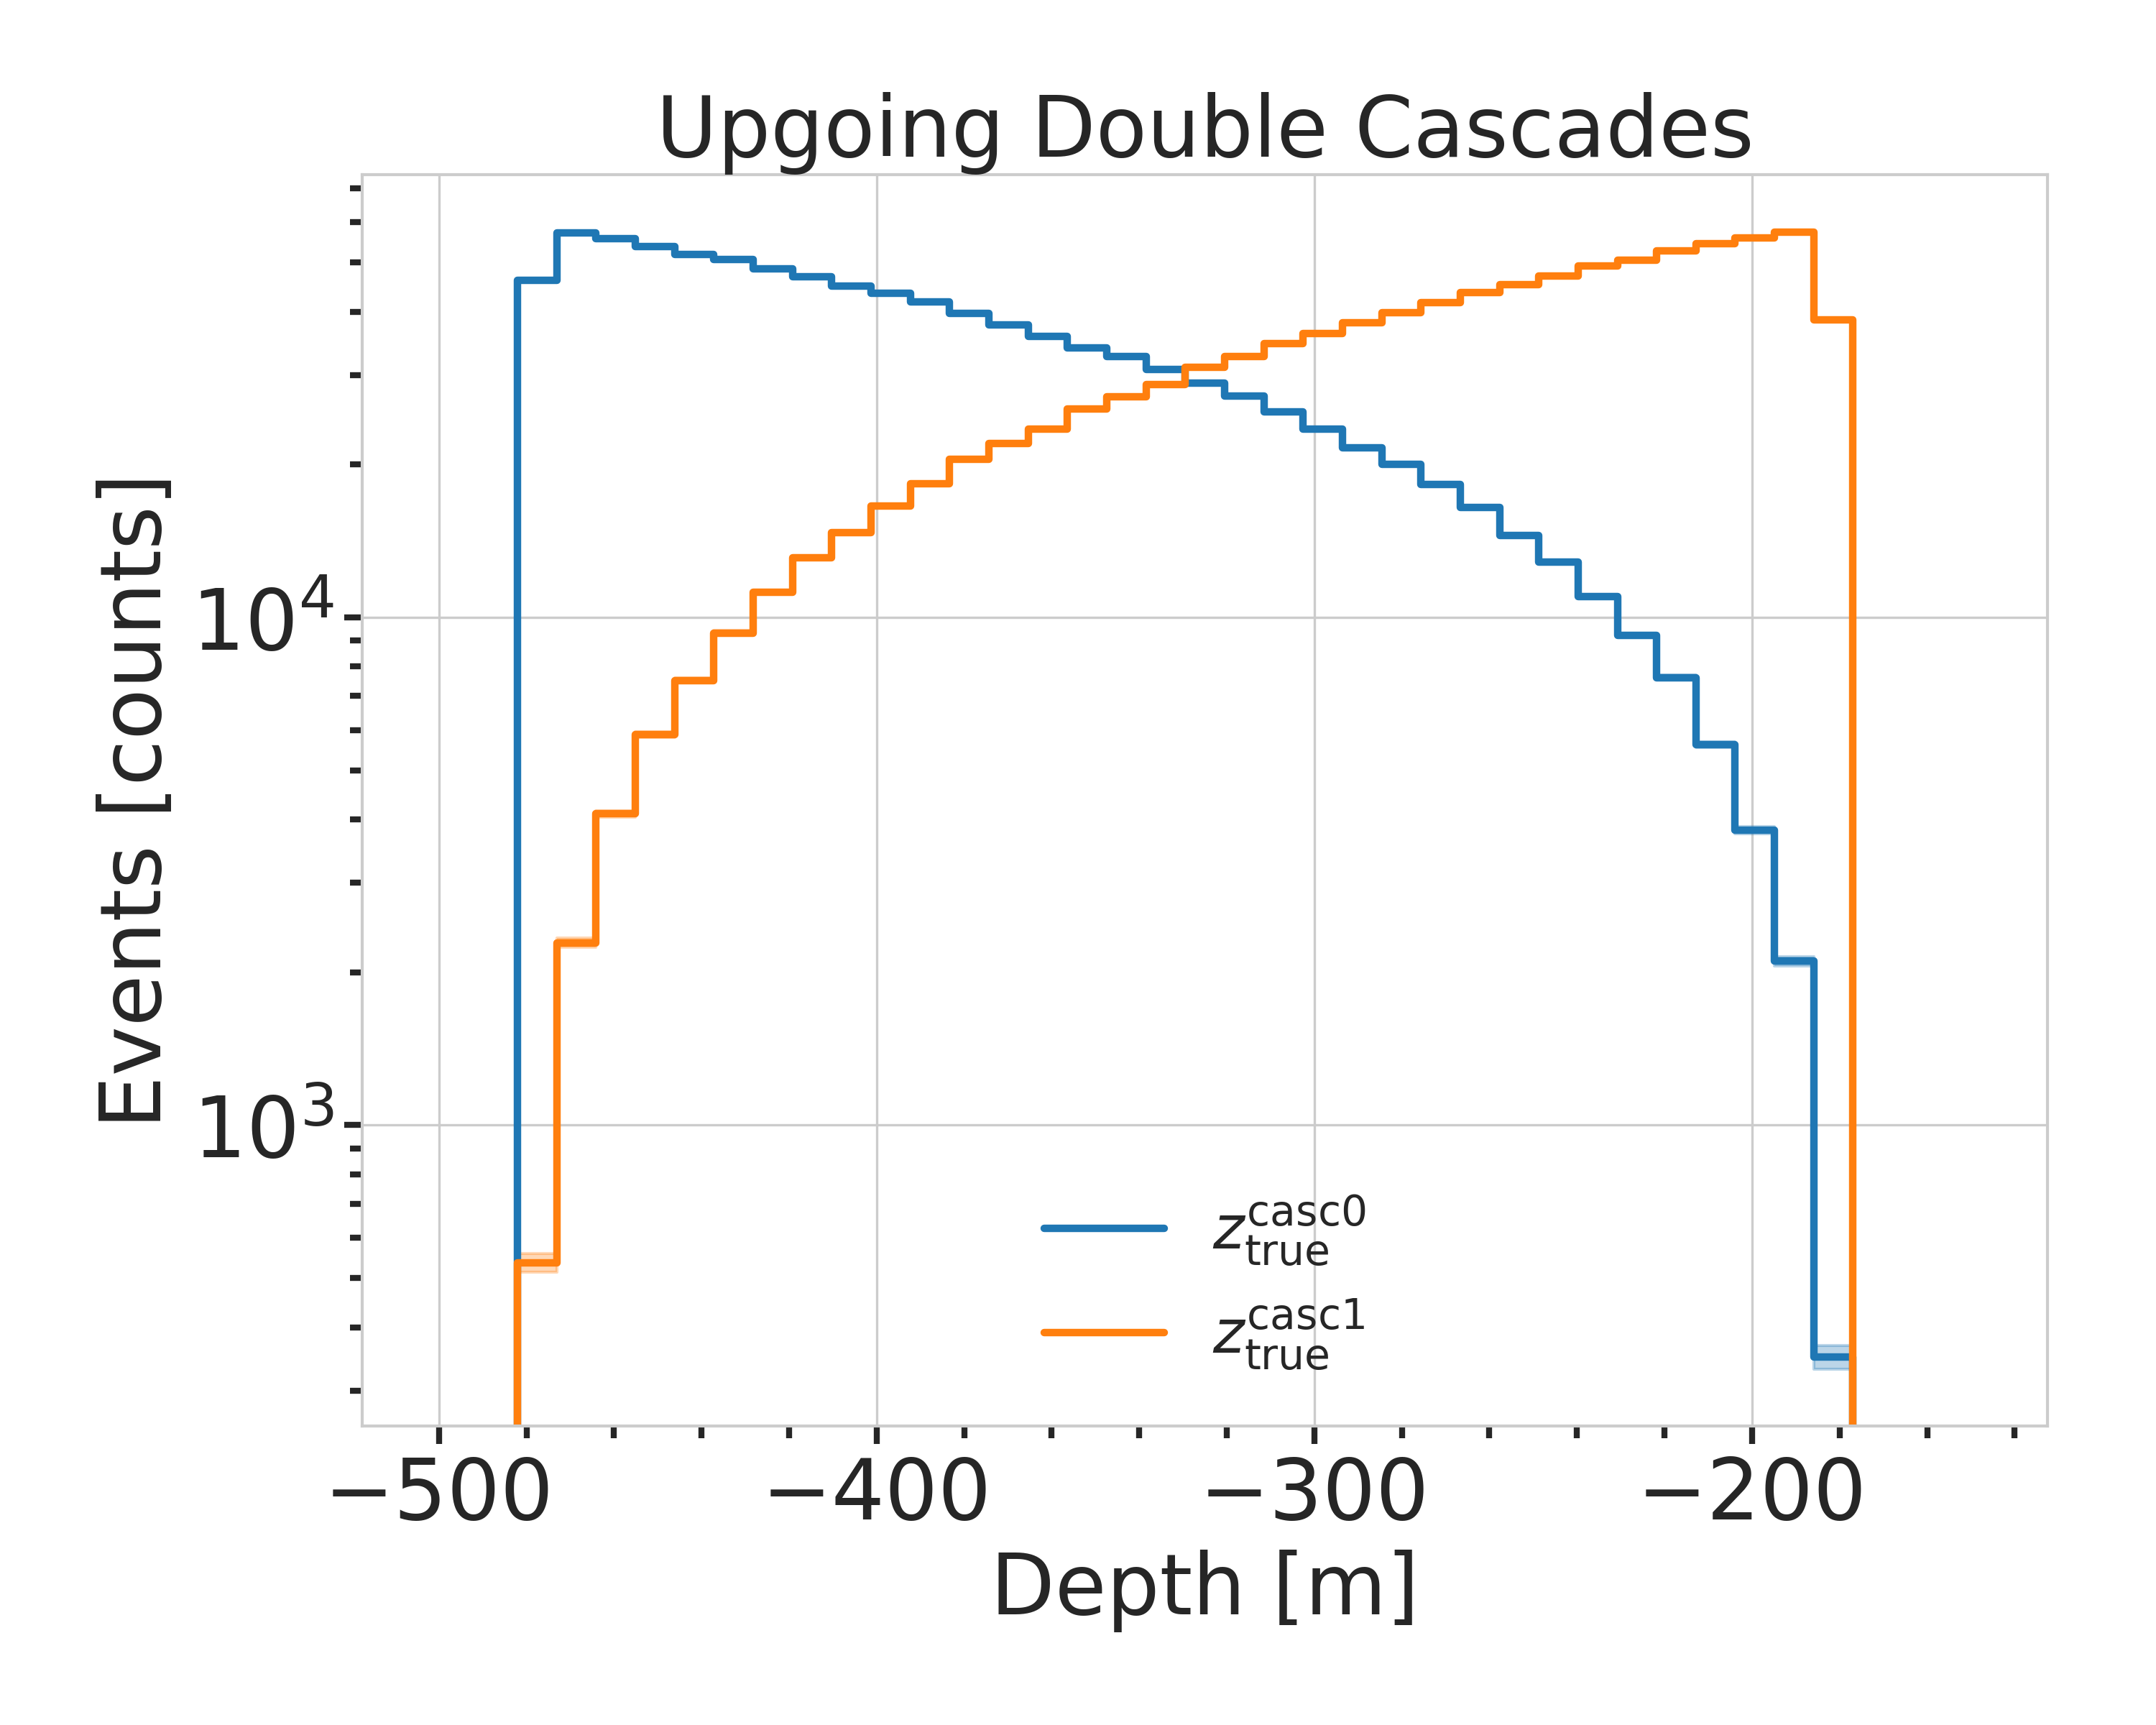
\includegraphics[width=0.49\linewidth]{figures/model_independent_simulation/gen_level/1_d_distr_depths_clipped.png}
    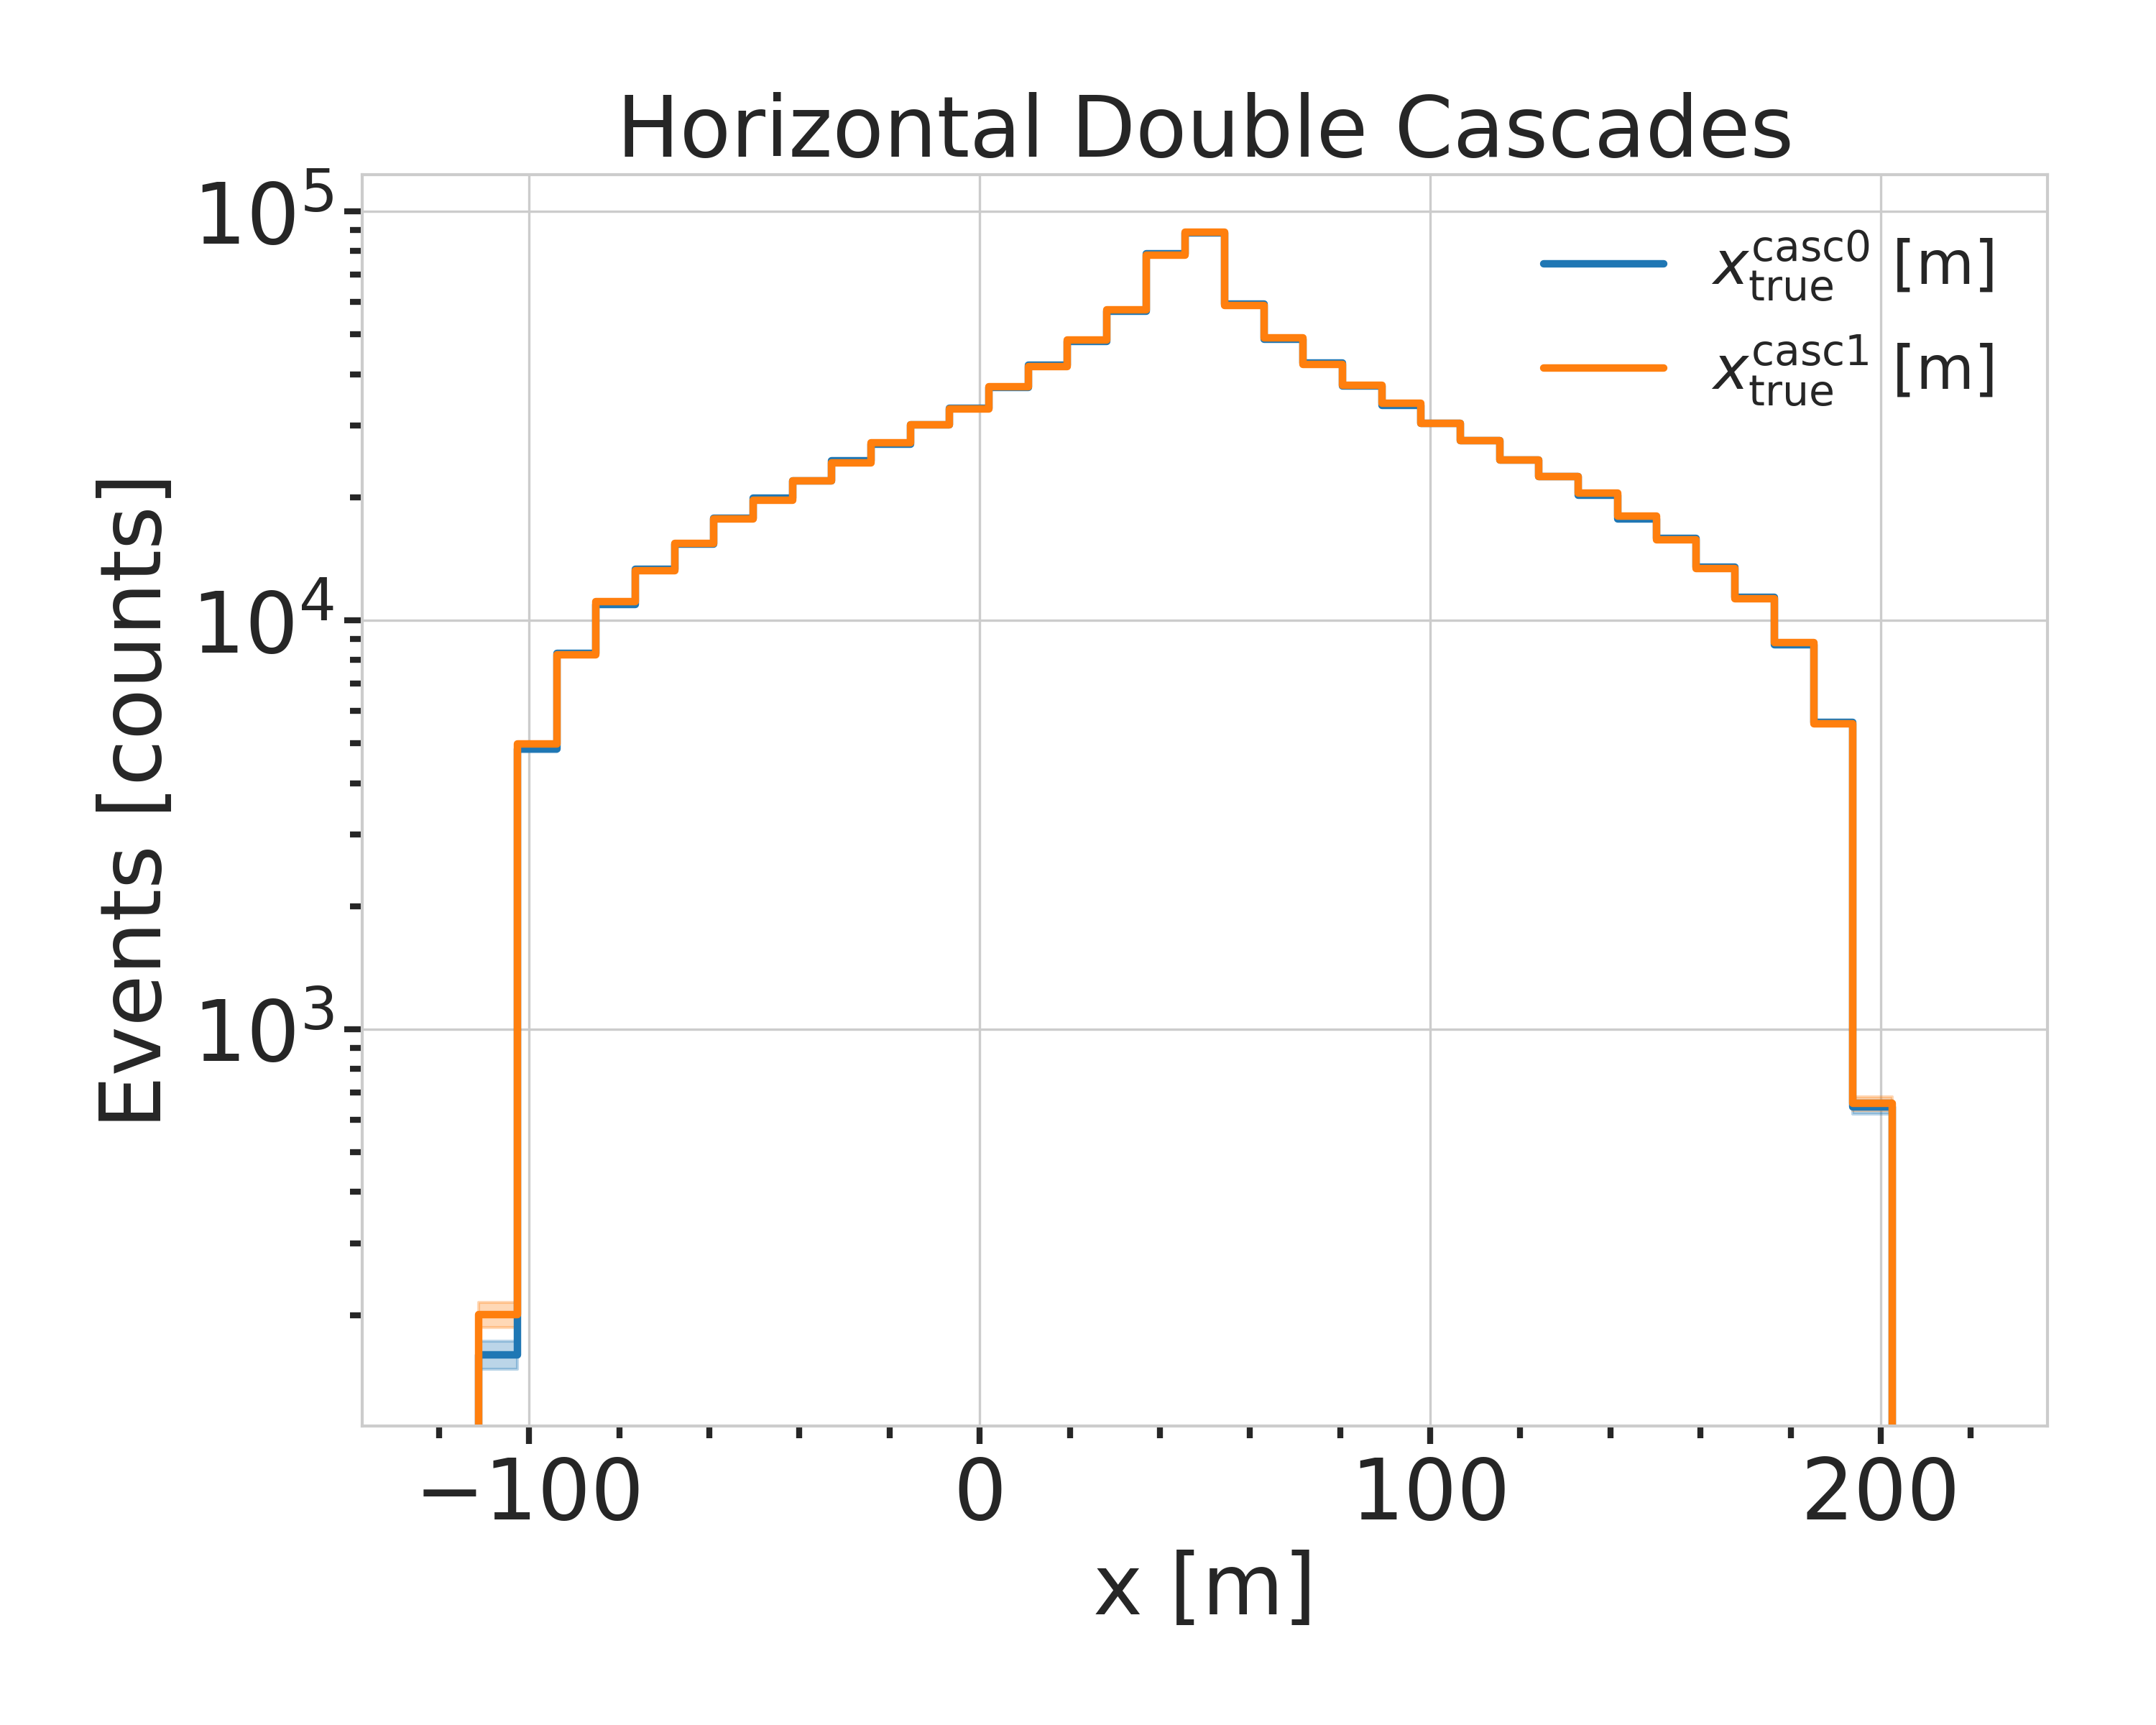
\includegraphics[width=0.49\linewidth]{figures/model_independent_simulation/gen_level/1_d_distr_xs_clipped.png}
    \caption[Simplified model independent simulation generation level distributions]{Generation level distributions of the simplistic simulation sets.Vertical positions (left) and horizontal positions (right) of both sets are shown.}
    \labfig{simplified_gen_distris_appendix}
\end{figure*}

\begin{figure*}
    \centering
    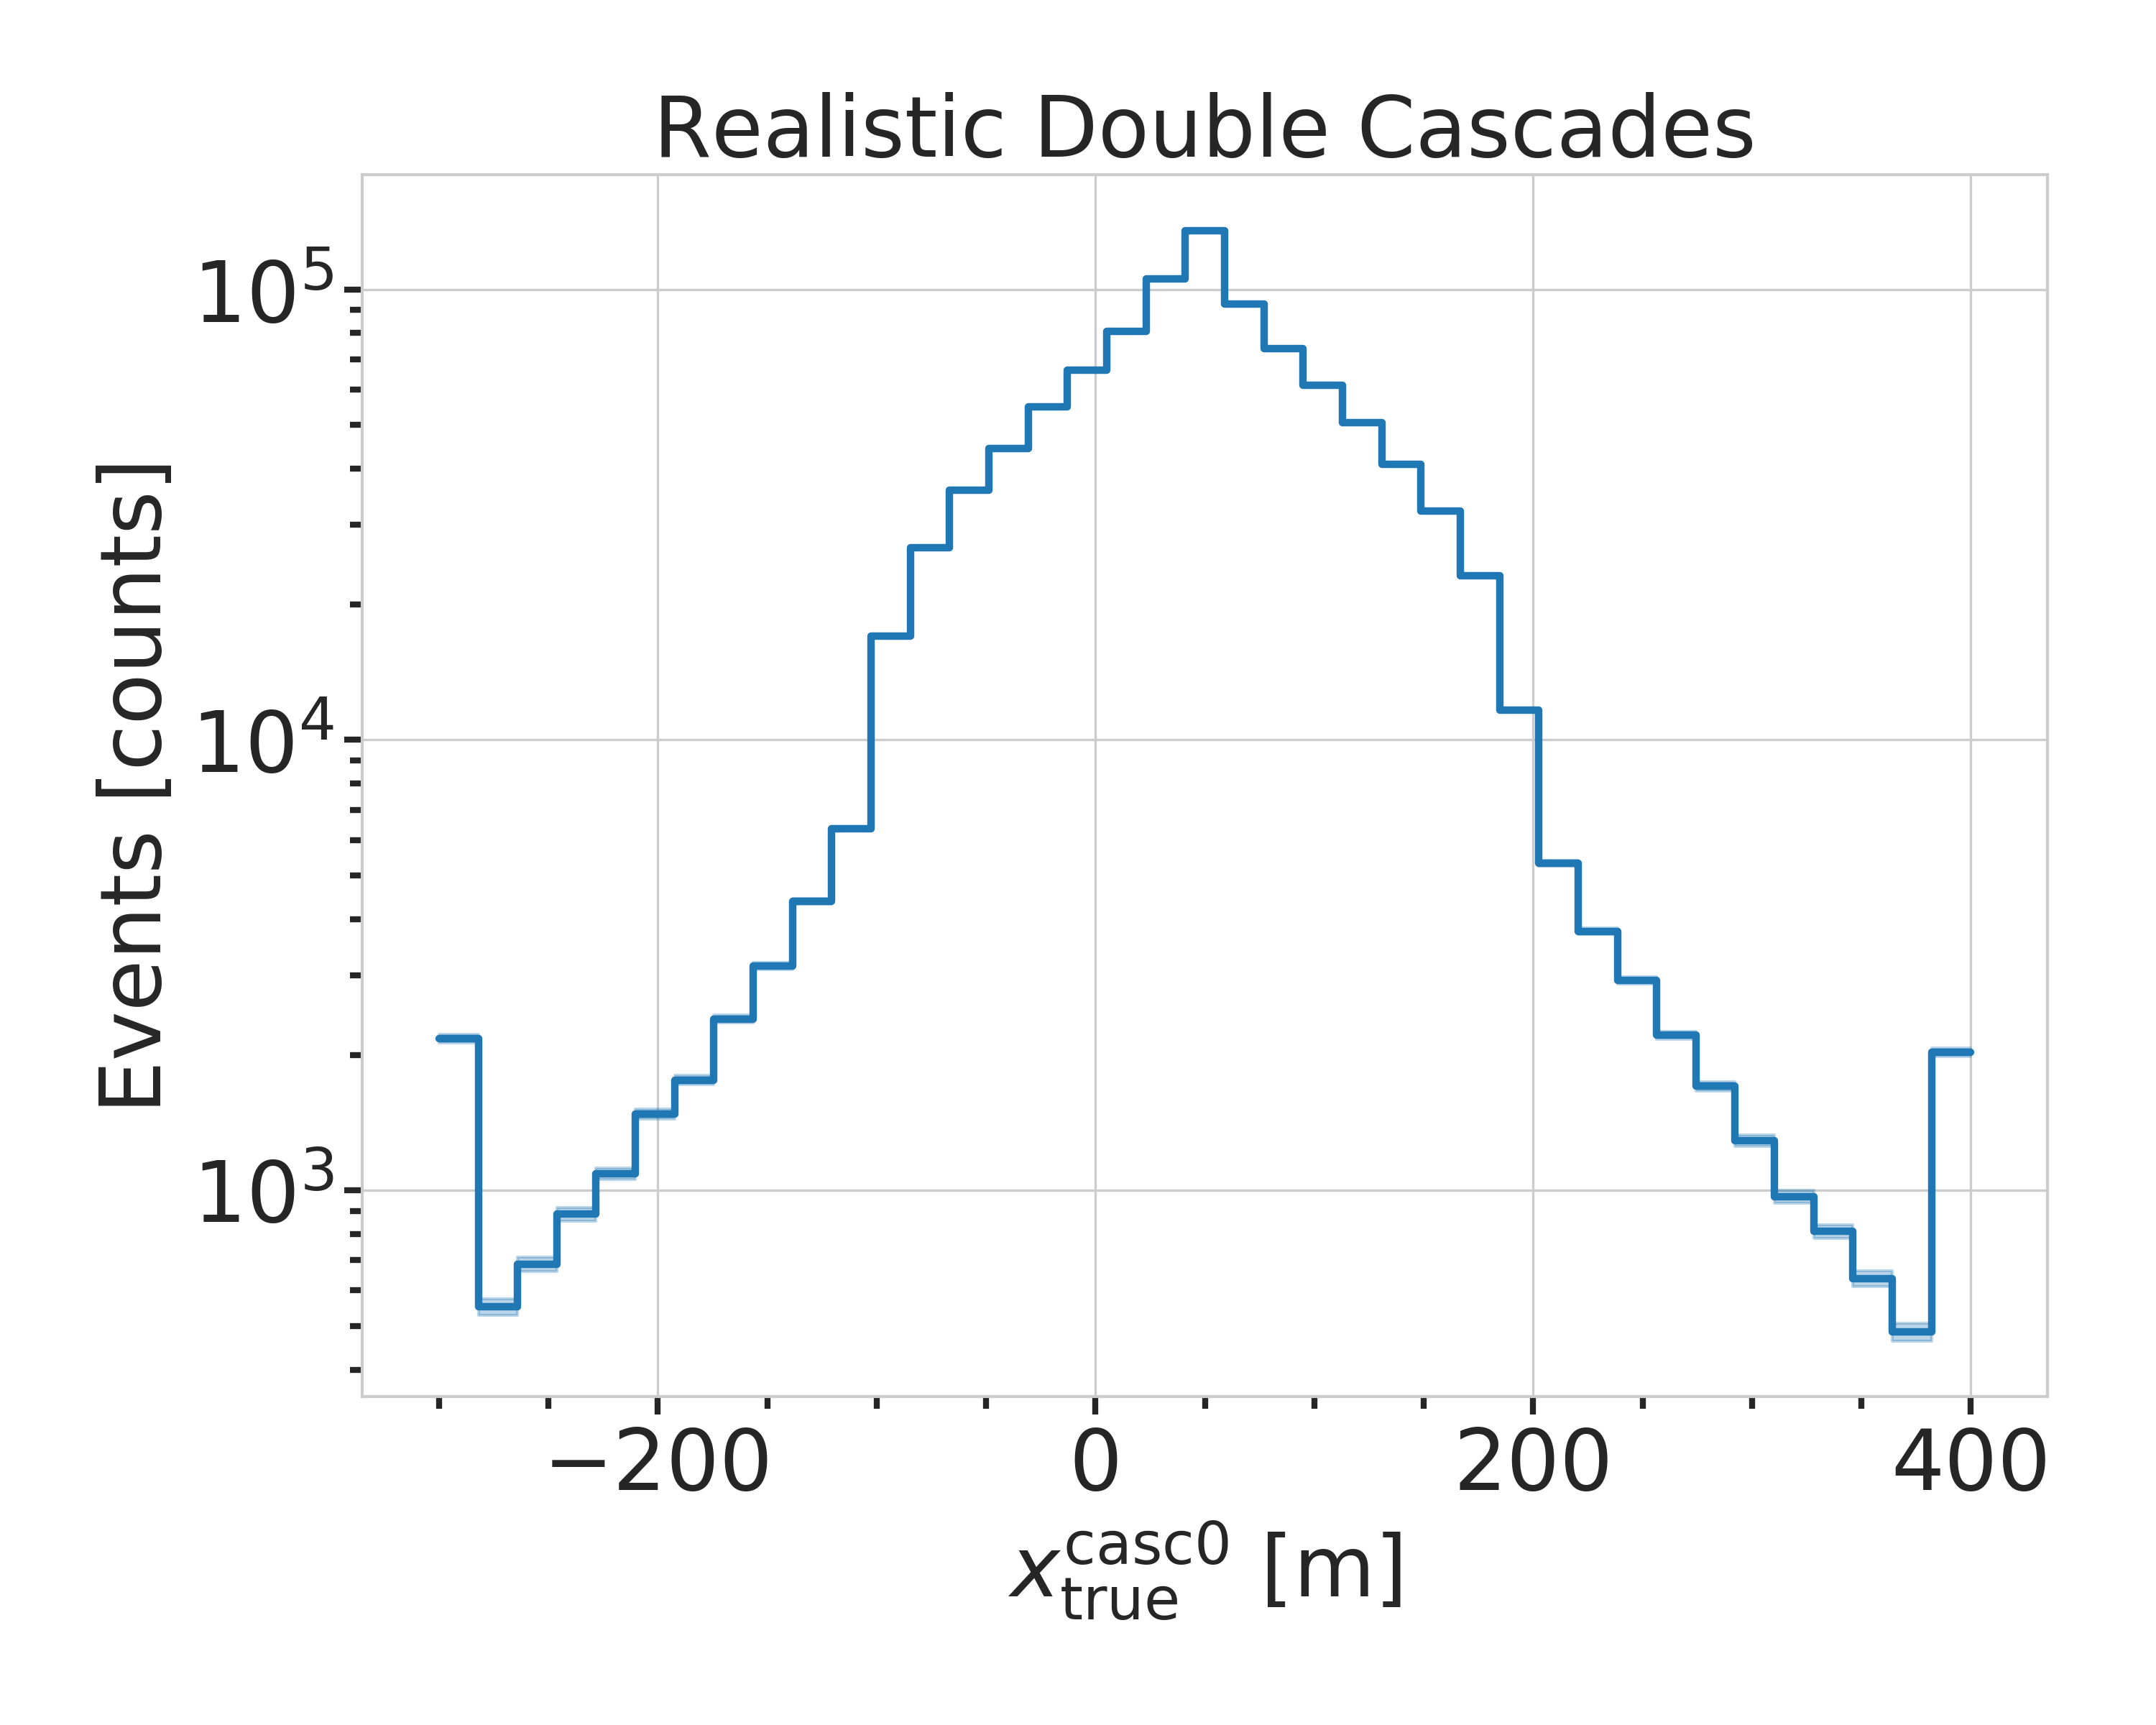
\includegraphics[width=0.49\linewidth]{figures/model_independent_simulation/gen_level/194603_gen_level_1_d_distr_casc0_true_x_clipped.png}
    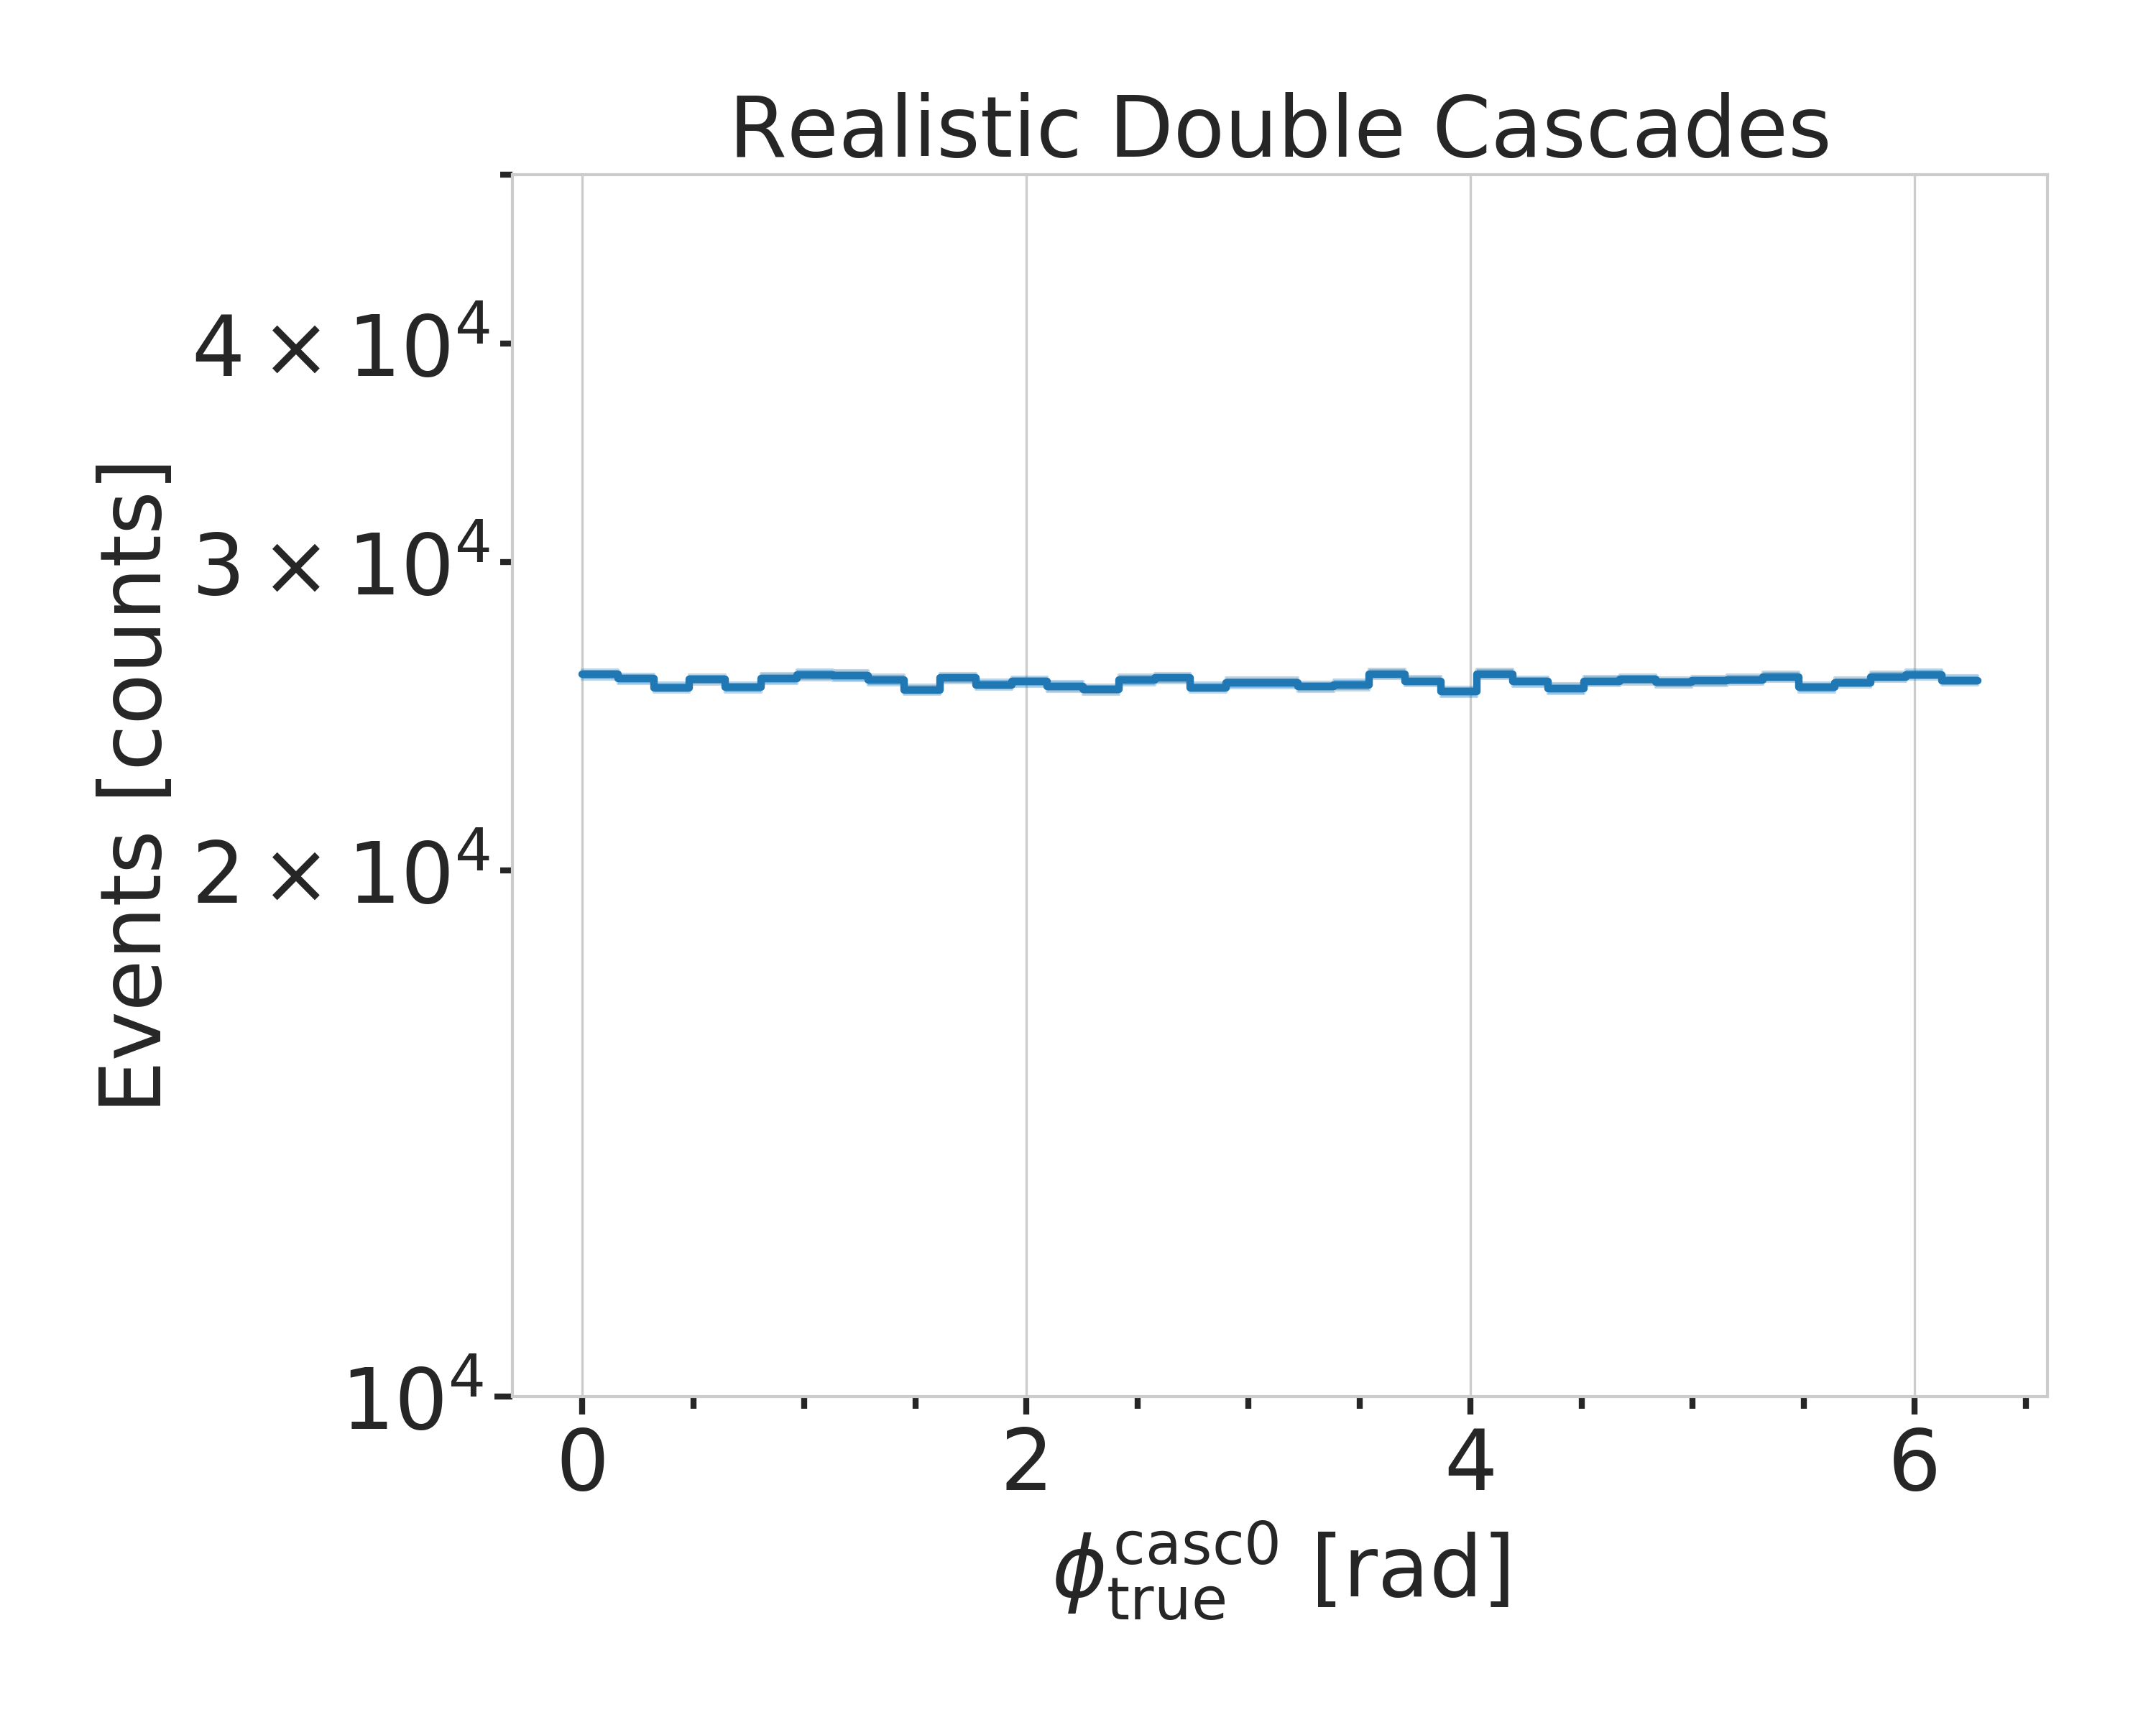
\includegraphics[width=0.49\linewidth]{figures/model_independent_simulation/gen_level/194603_gen_level_1_d_distr_casc0_true_azimuth_clipped.png}
    \caption[Realistic model independent simulation generation level distributions]{Generation level distributions of the simplistic realistic set. Shown are the cascade $x, y, z$ positions (left) and direction angles (right).}
    \labfig{realistic_gen_distris_appendix}
\end{figure*}

\section{Model Dependent Simulation Distributions} \labsec{model_dependent_simulation_appendix}

\begin{figure*}[h]
    \centering
    \begin{subfigure}{0.49\linewidth}
        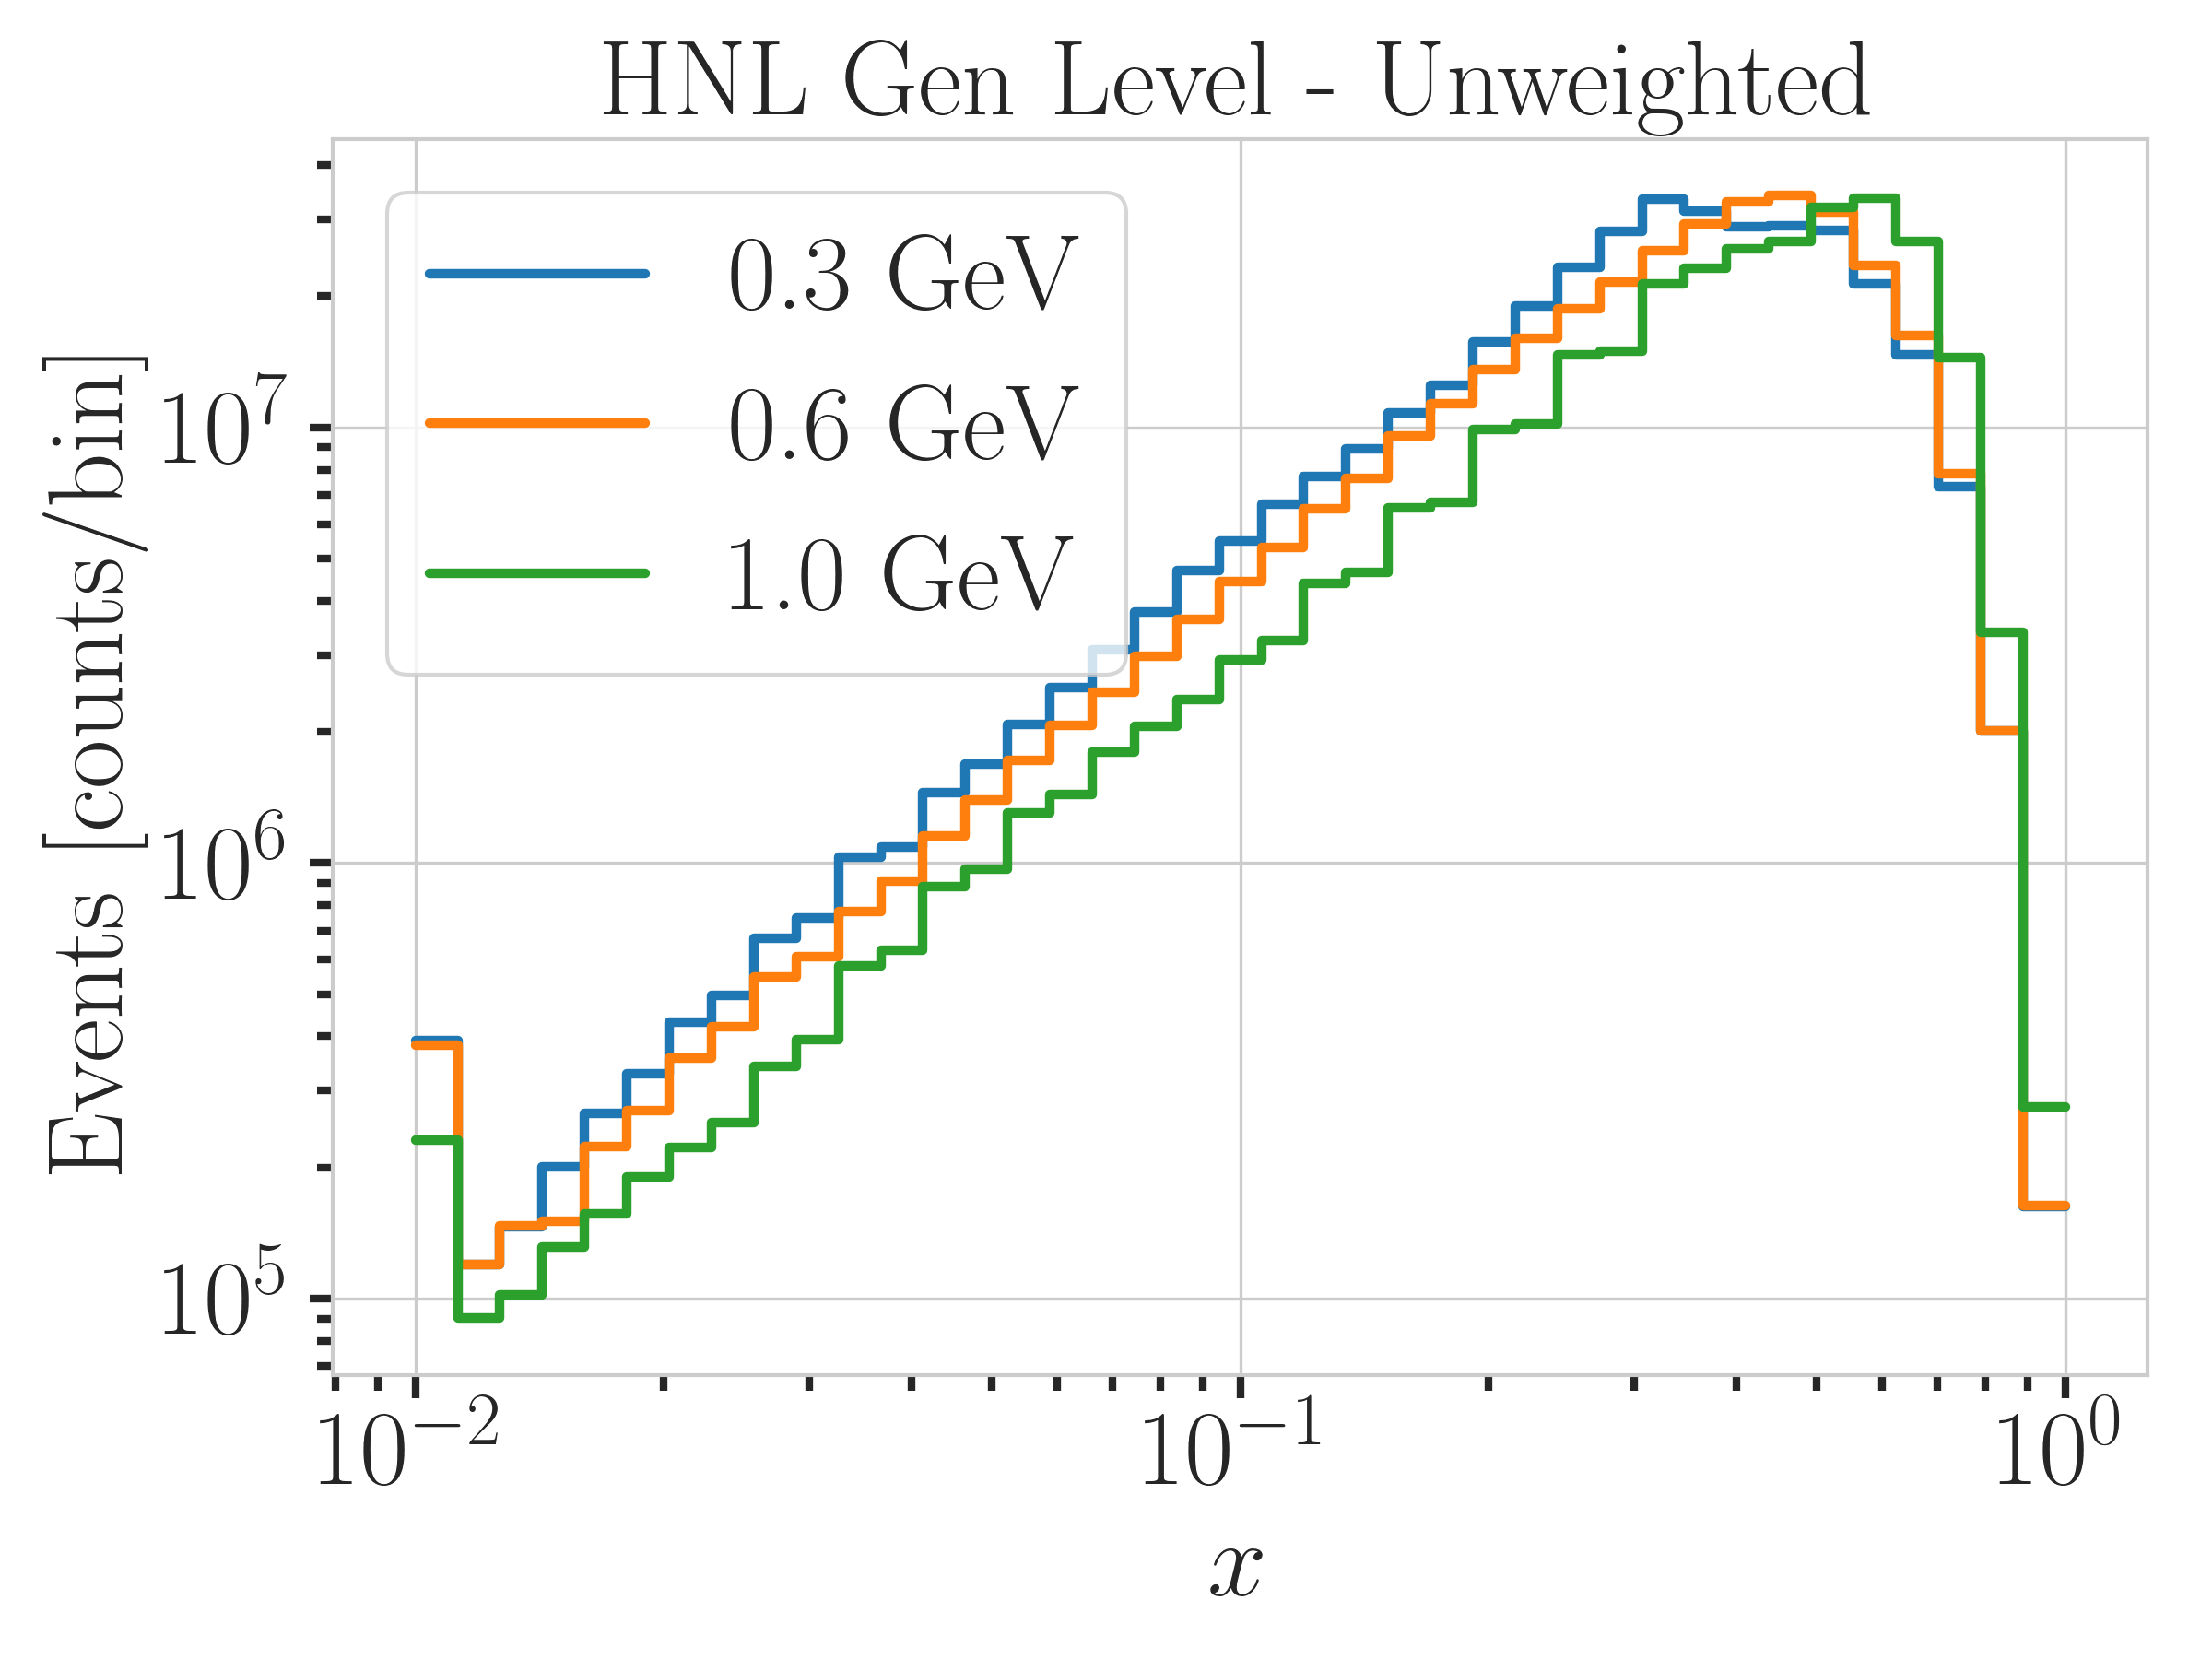
\includegraphics{figures/hnl_simulation/generation/1_d_distr_finalStateX_gen_level_unweighted.png}
        \caption{Bjorken x}
    \end{subfigure}
    \begin{subfigure}{0.49\linewidth}
    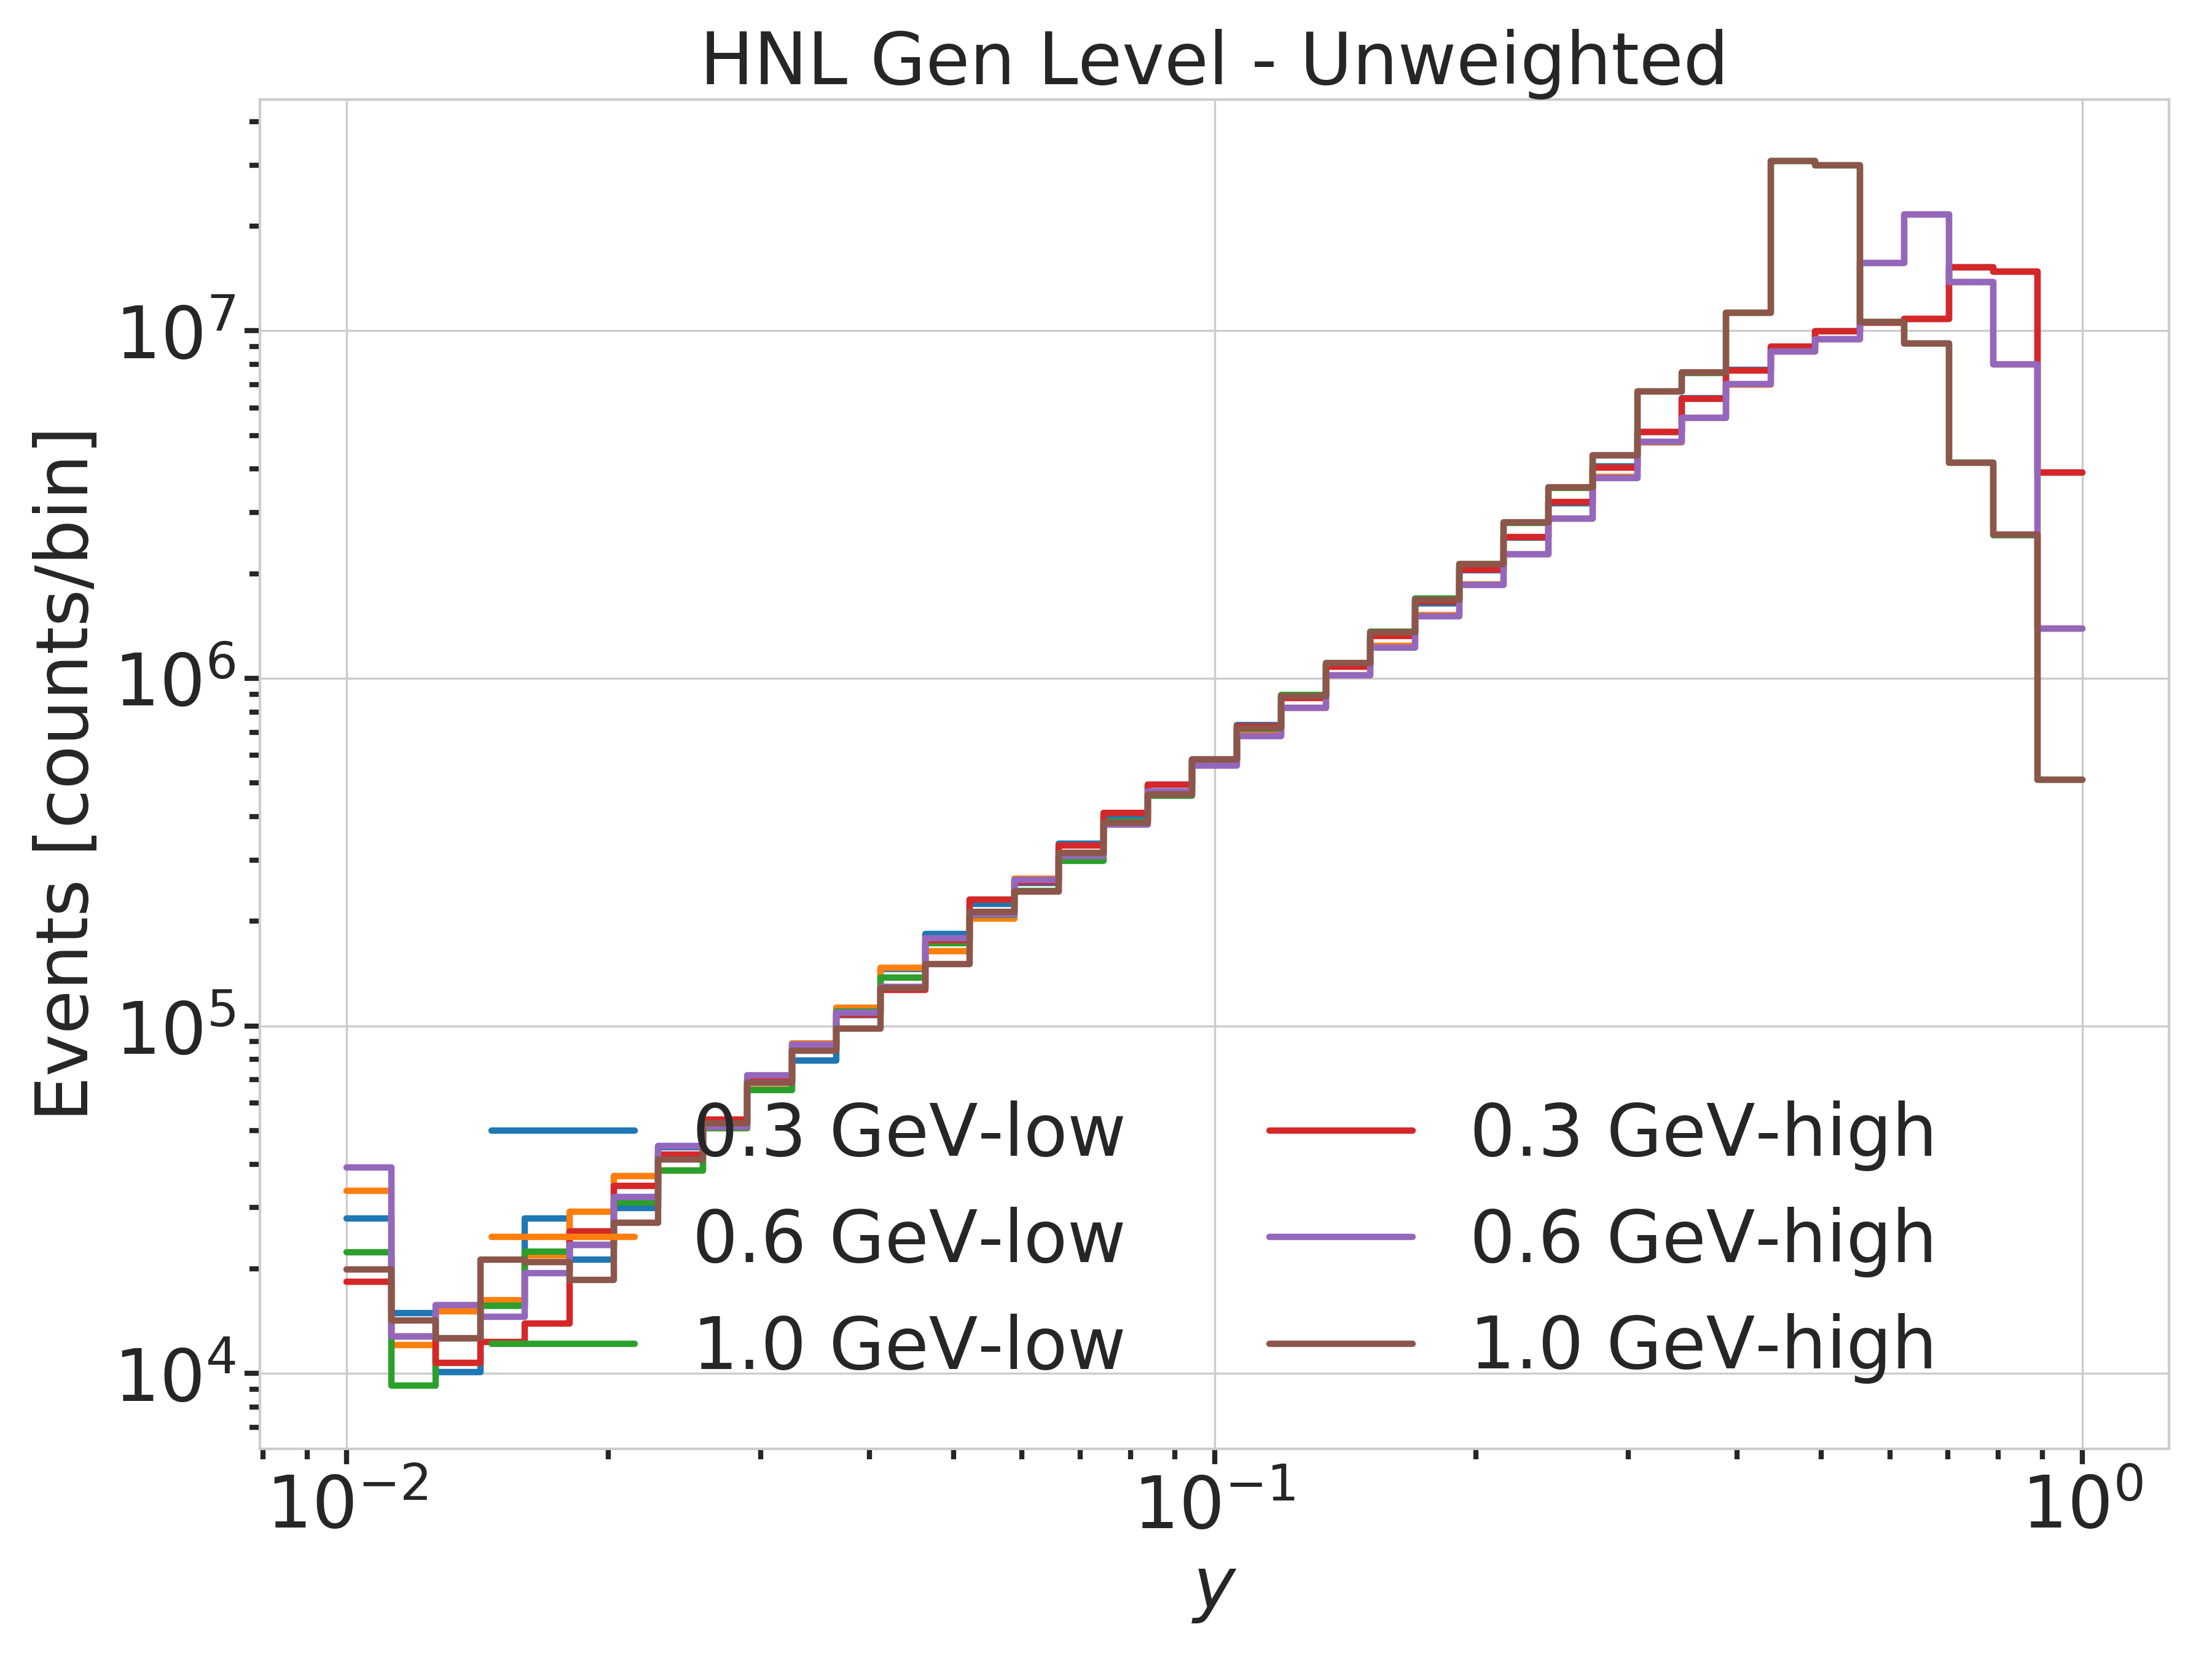
\includegraphics{figures/hnl_simulation/generation/1_d_distr_finalStateY_gen_level_unweighted.png}
        \caption{Bjorken y}
    \end{subfigure}
    \caption[Model dependent simulation generation level distributions]{Generation level distributions of the model dependent simulation.}
    \labfig{hnl_gen_distris_appendix}
\end{figure*}


\setchapterstyle{lines}
\chapter{Analysis Checks}
\labch{analysis_checks}


\section{Minimization Robustness} \labsec{asimov_inject_recover_appendix}

\reffig{asimov_inject_recover_appendix} shows additional Asimov inject/recover tests for the \SI{0.3}{\gev} and\SI{1.0}{\gev} mass sets. The tests were described in \refsec{asimov_inject_recover}.

\begin{figure*}[h]
    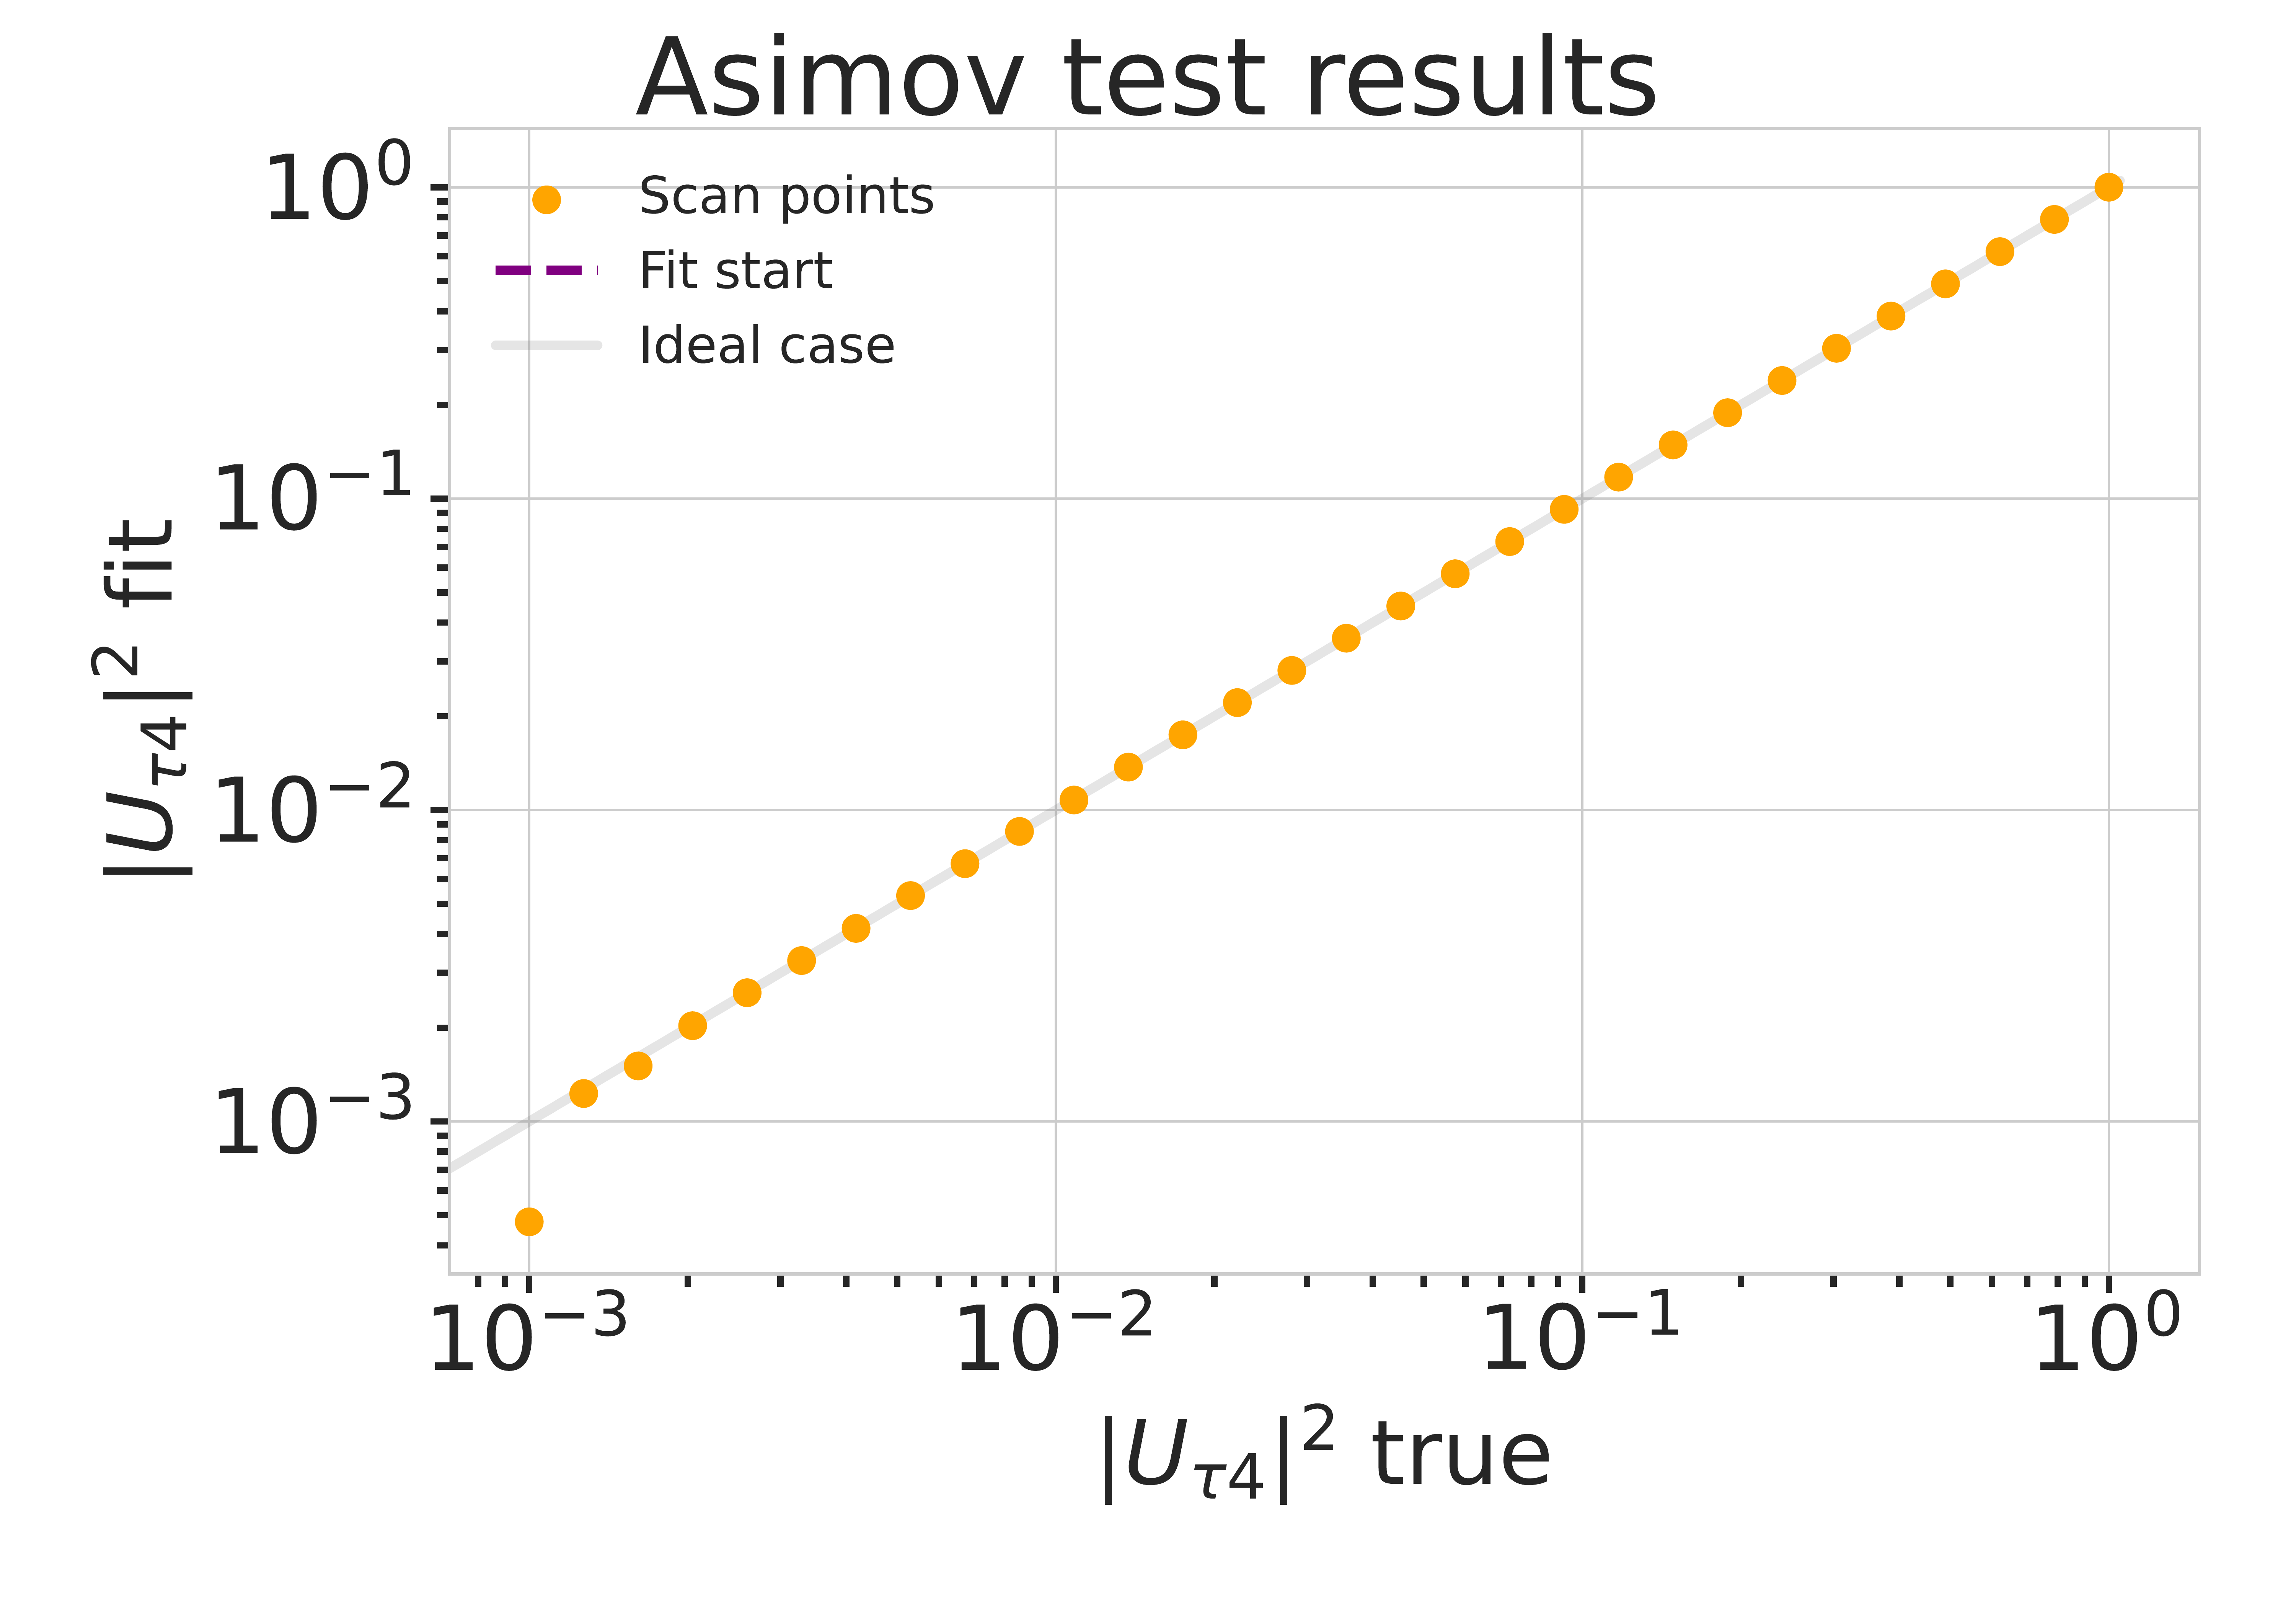
\includegraphics[width=0.49\linewidth]{figures/results/checks/asimov_scan_0.3_GeV-01.png}
    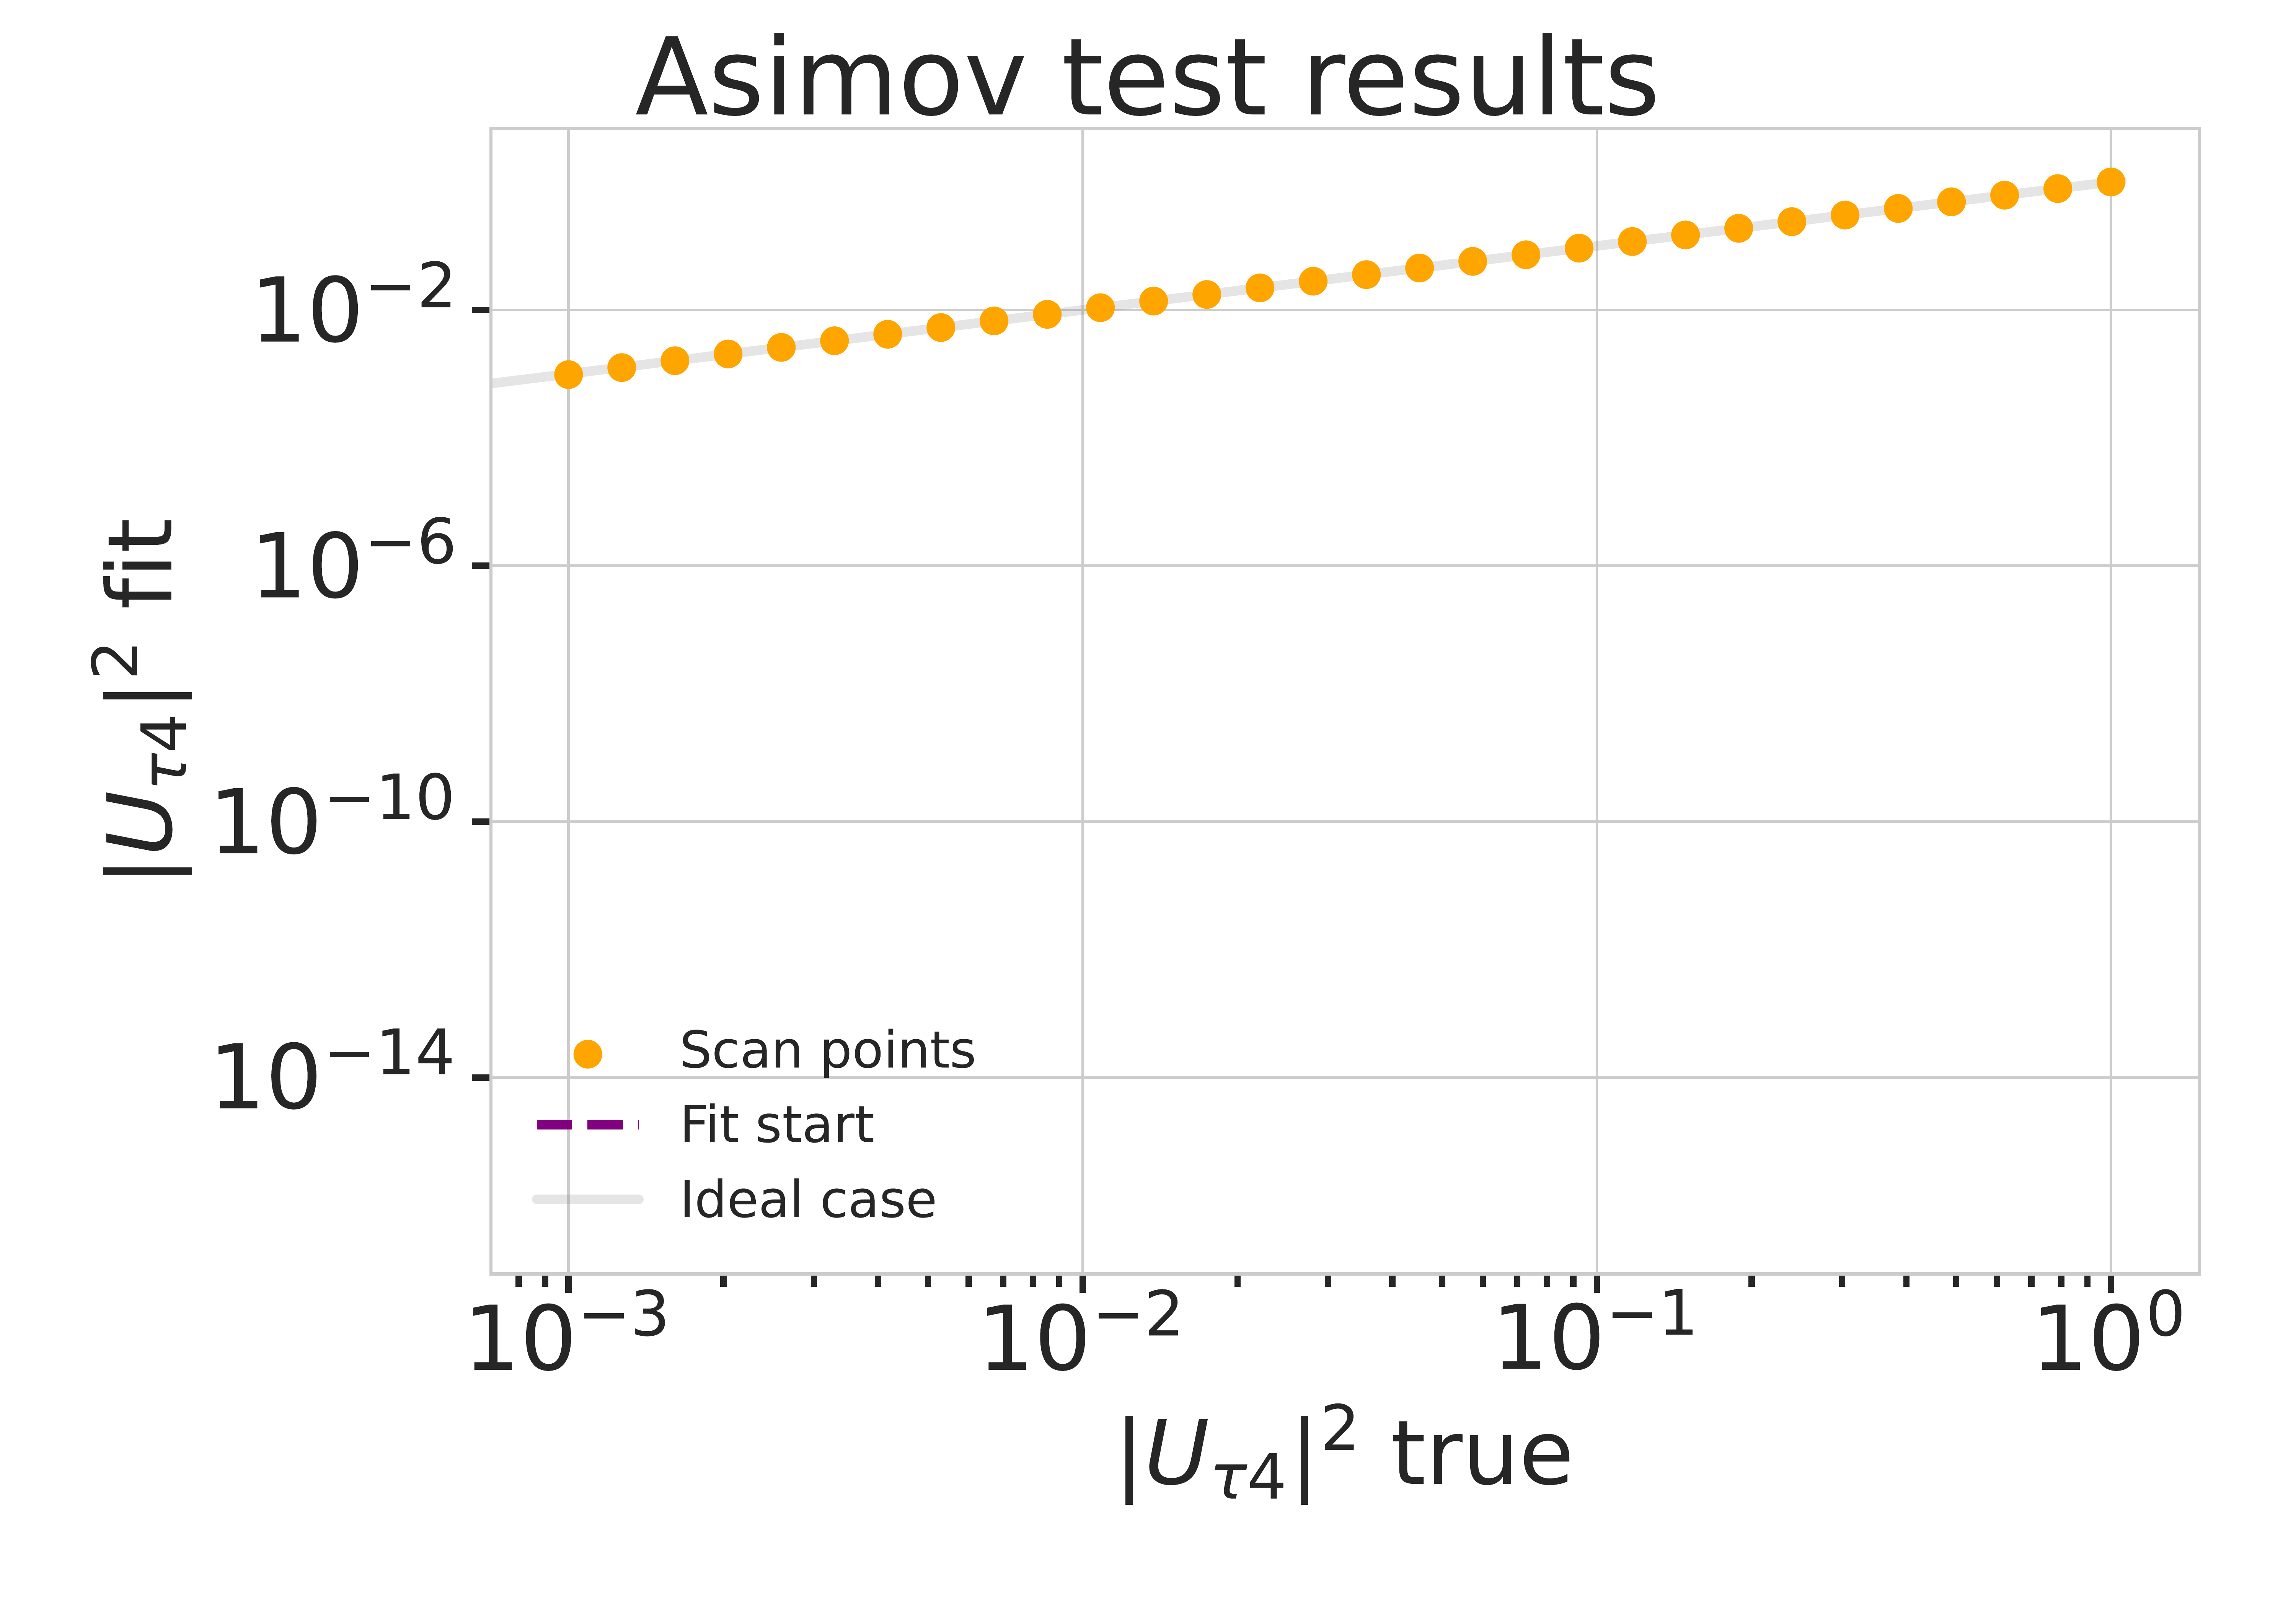
\includegraphics[width=0.49\linewidth]{figures/results/checks/asimov_scan_1.0_GeV-01.png}
	\caption[Asimov inject/recover test (\SI{0.3}{\gev}, \SI{1.0}{\gev})]{Asimov inject/recover test for the \SI{0.3}{\gev} (left) and \SI{1.0}{\gev} (right) mass sets. Mixing values between $10^{-3}$ and $10^{0}$ are injected and fit back with the full analysis chain. The injected parameter is always recovered within the statistical uncertainty.}
    \labfig{asimov_inject_recover_appendix}
\end{figure*}


% \ection{Sensitivities}

% \begin{figure}[h]
%     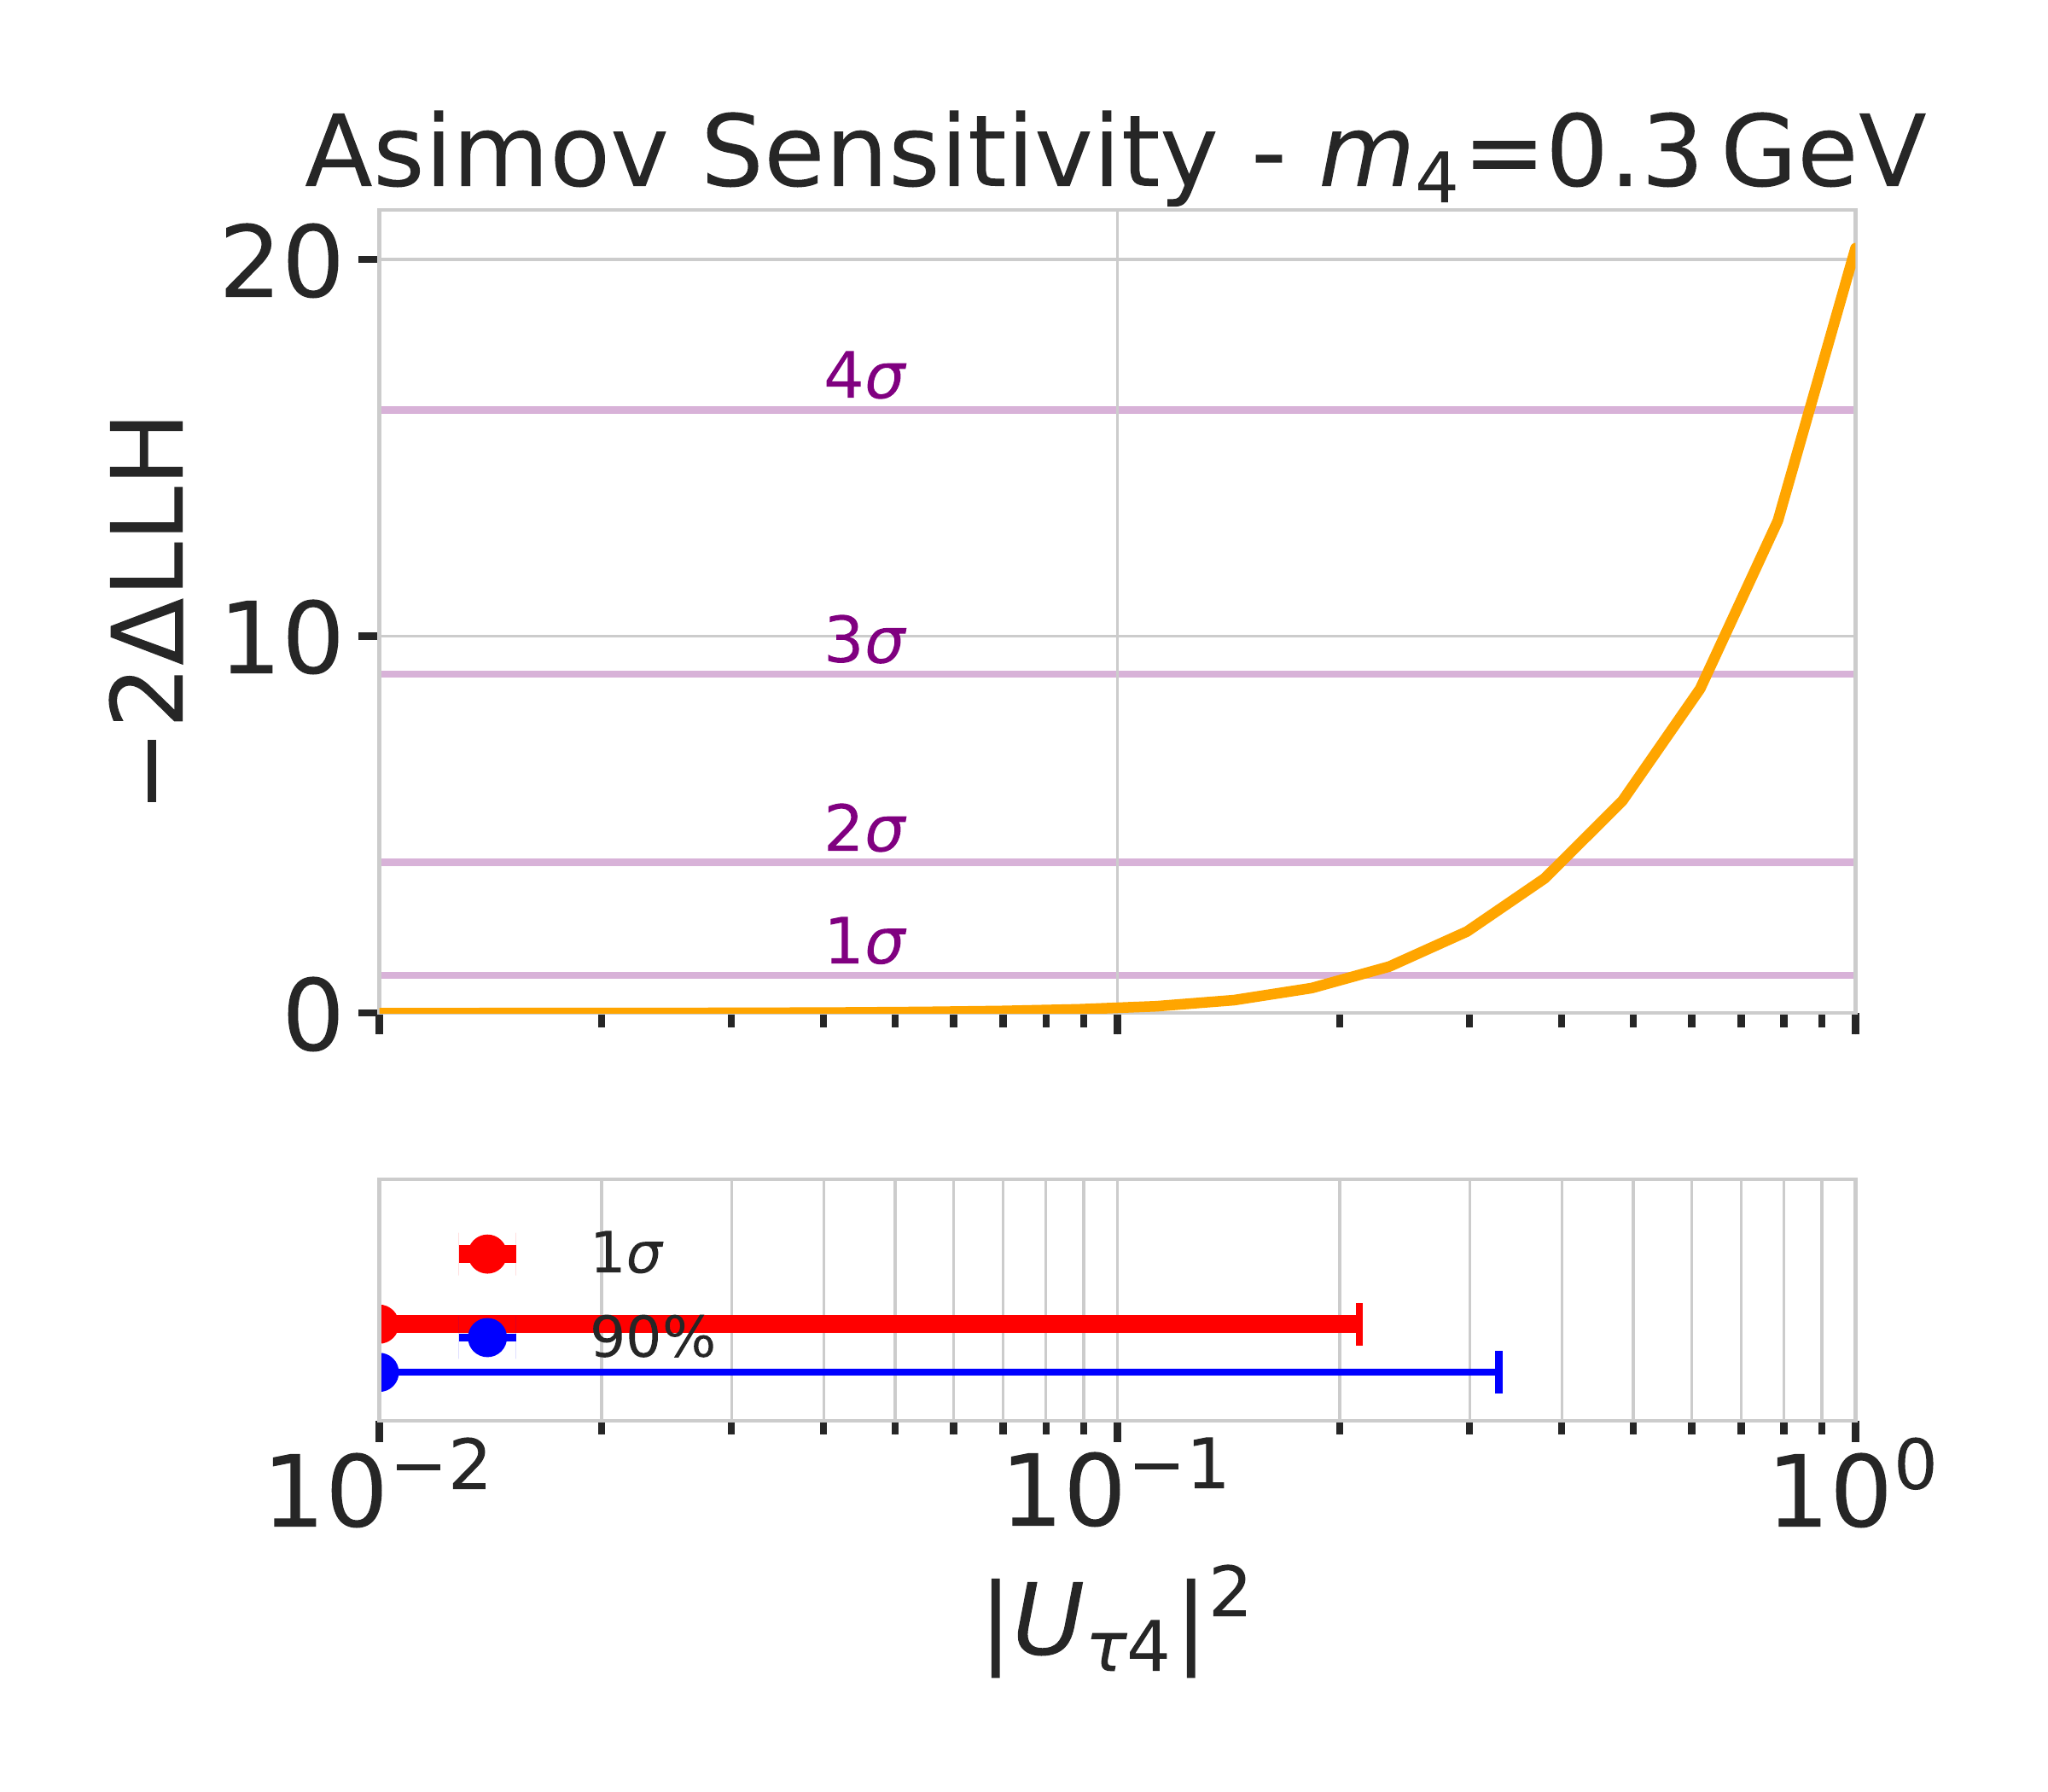
\includegraphics[width=0.49\linewidth]{figures/results/checks/sensitivity_scan_0.3_GeV-1.png}
%     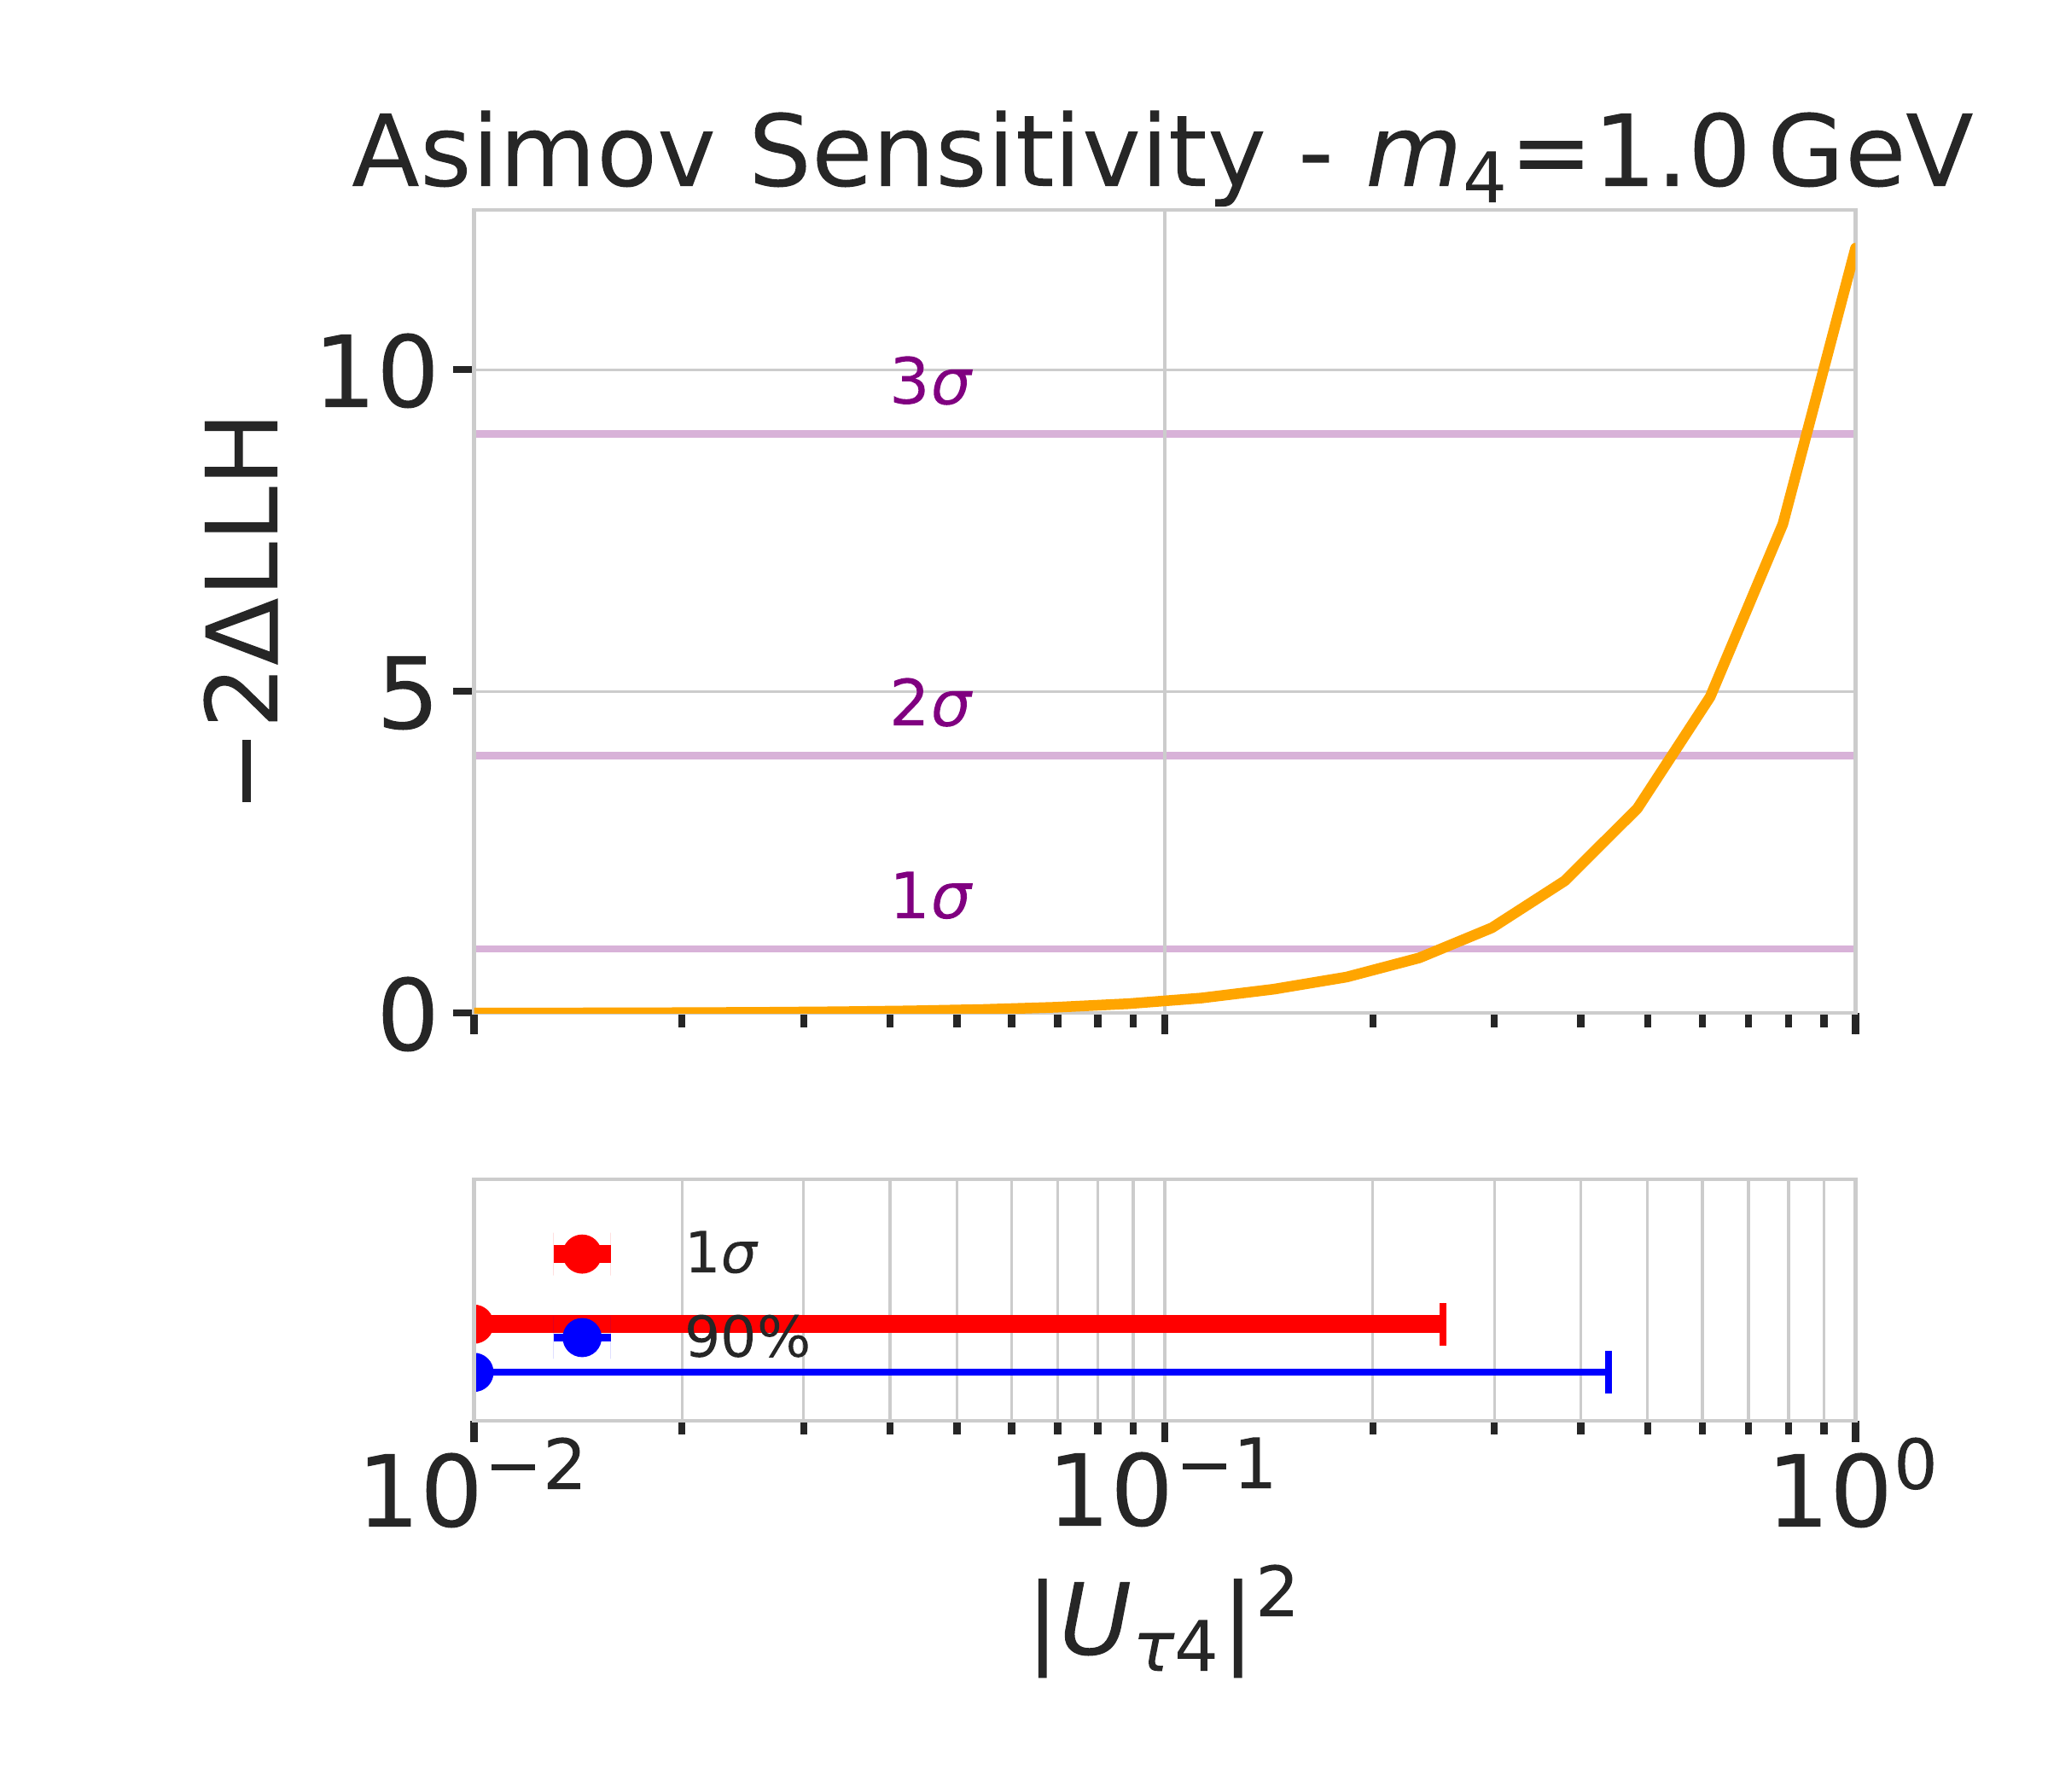
\includegraphics[width=0.49\linewidth]{figures/results/checks/sensitivity_scan_1.0_GeV-1.png}
% 	\caption[Sensitivity scan (\SI{0.3}{\gev}, \SI{1.0}{\gev})]{Sensitivity scan for the \SI{0.3}{\gev} (left) and \SI{1.0}{\gev} (right) mass sets.}
%     \labfig{sensitivity_scan_0.6_GeV}
% \end{figure}


\subsection{Ensemble Tests} \labsec{pseudo_data_ensemble_appendix}

\reffig{pseudo_data_ensemble_appendix} shows additional TS distributions from pseudo-data trials and the observed TS from the fit to the data for the ensemble for the \SI{0.3}{\gev} and\SI{1.0}{\gev} mass sets. The tests were described in \refsec{pseudo_data_ensemble}.


\begin{figure*}[h]
    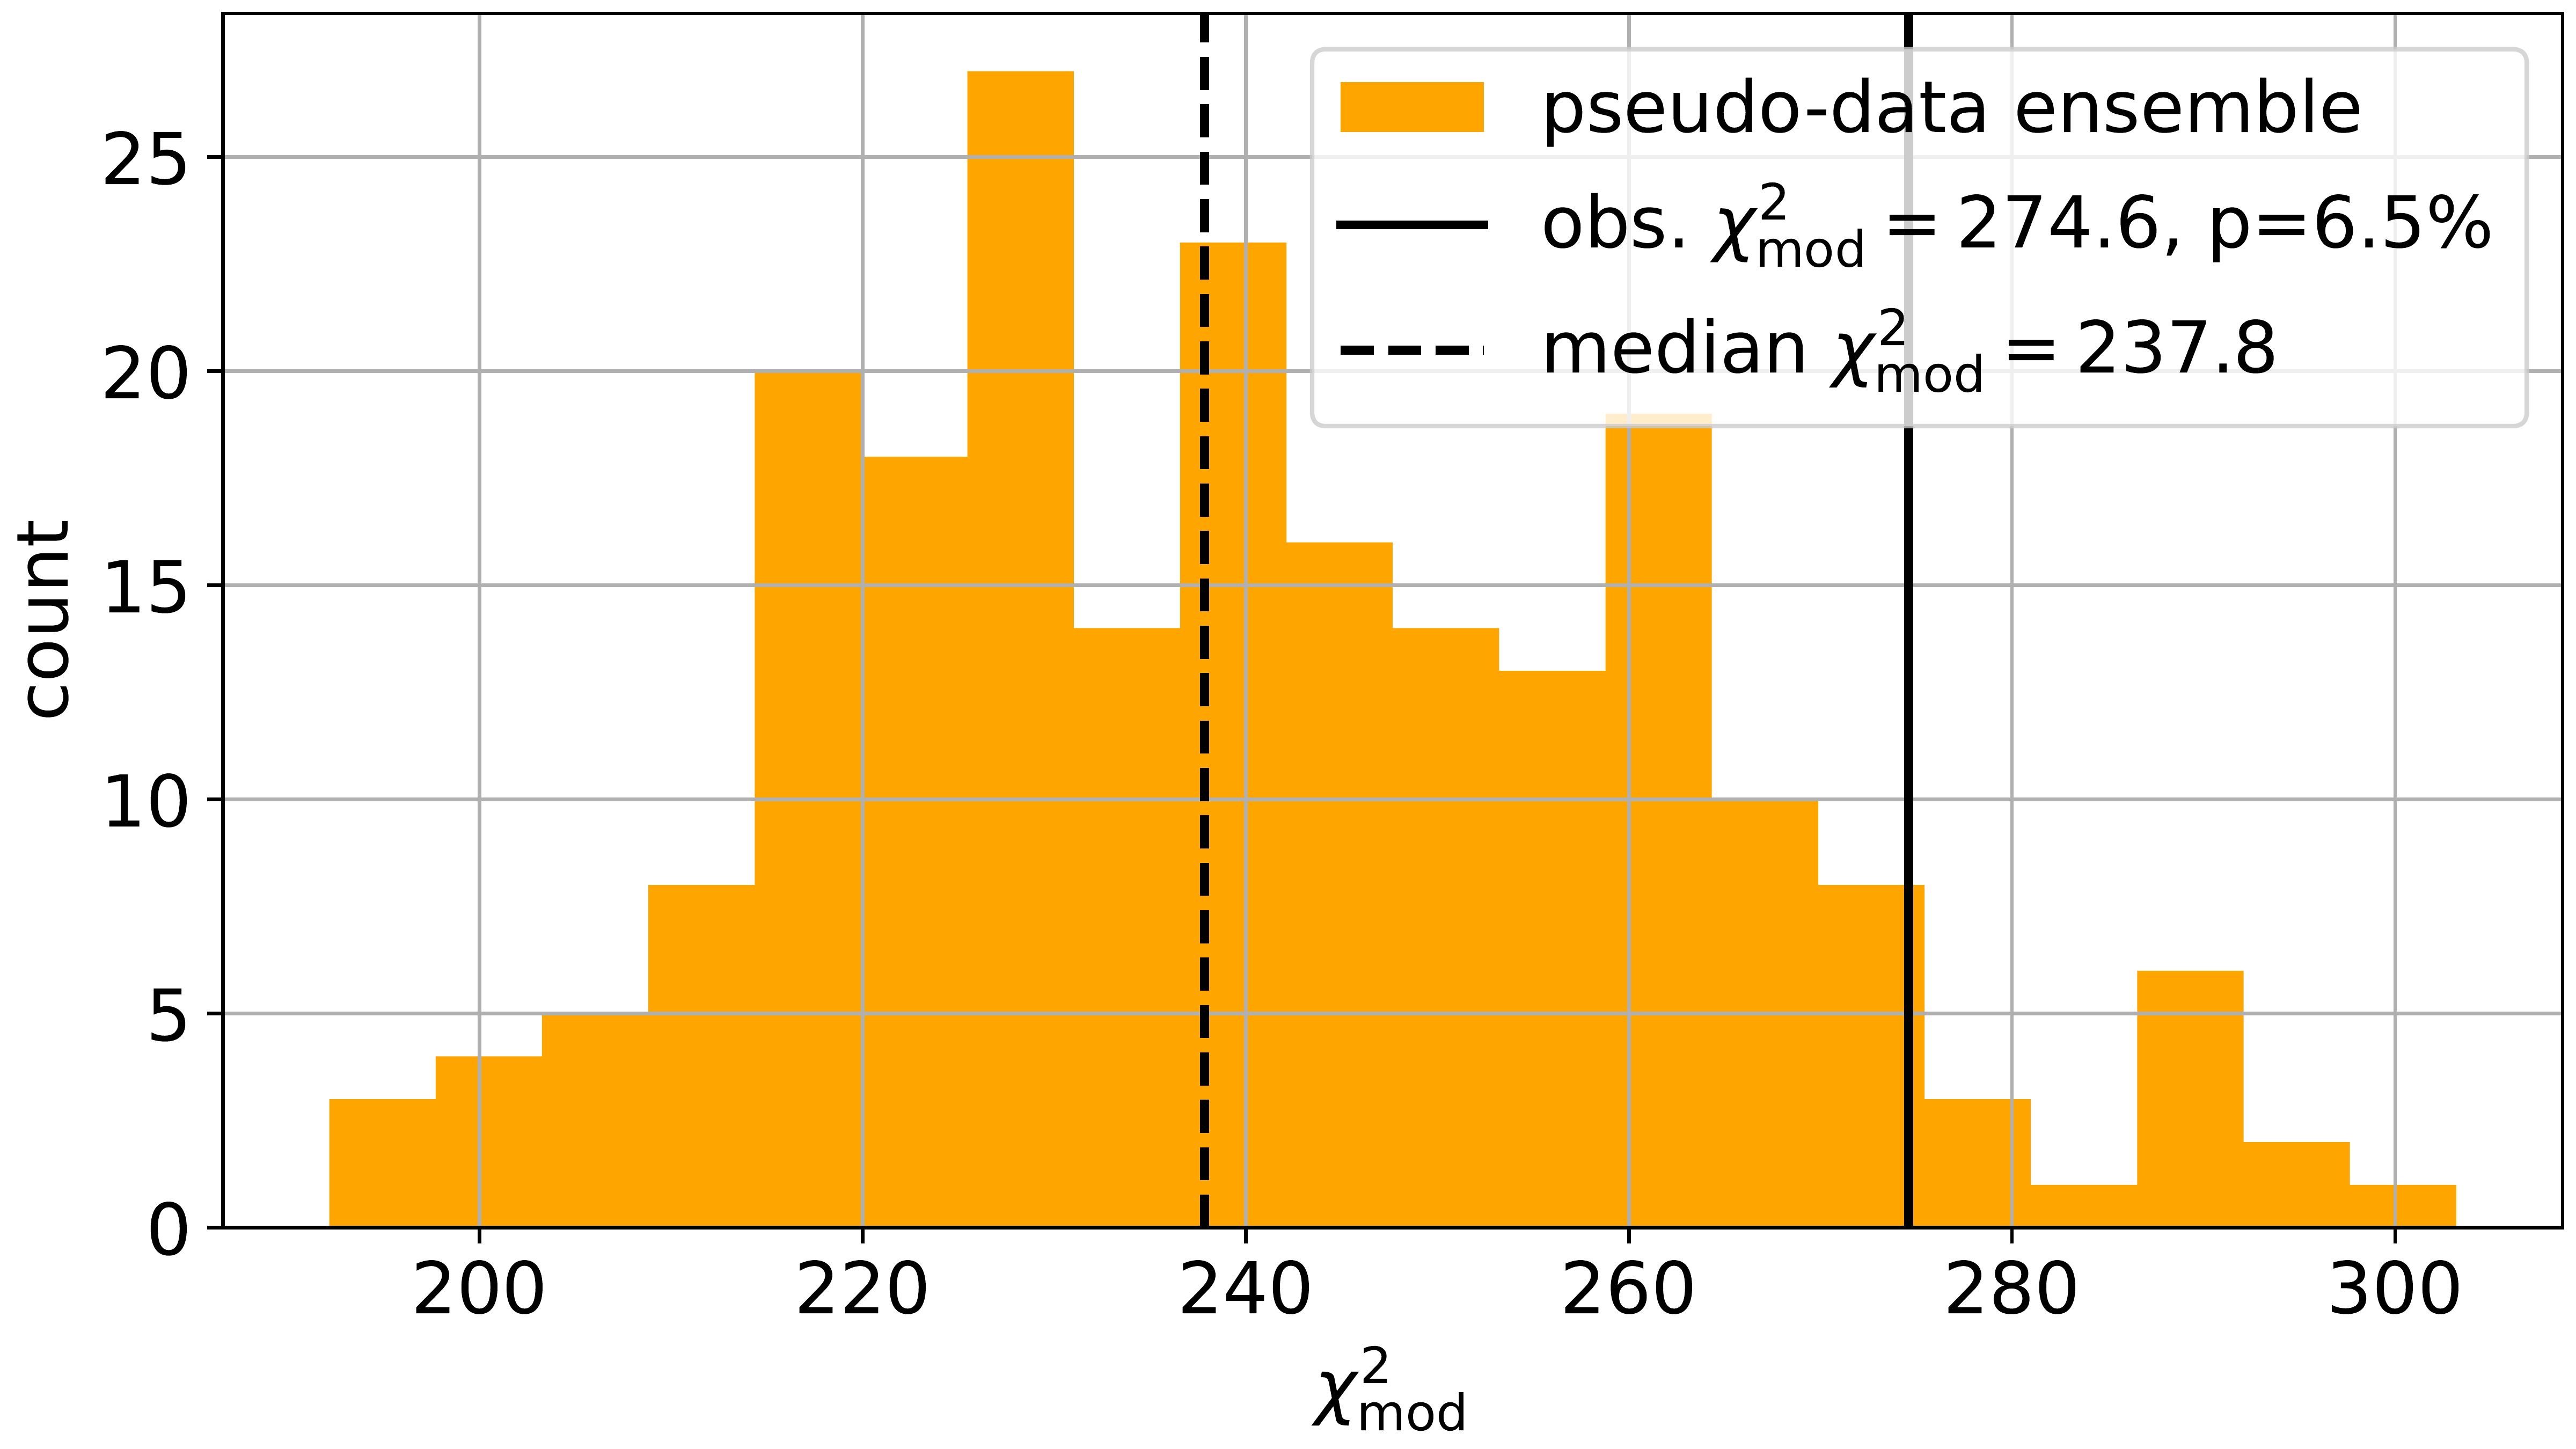
\includegraphics[width=0.49\linewidth]{figures/results/checks/full_blind_fit_0.3_GeV_step_3_4-1.png}
    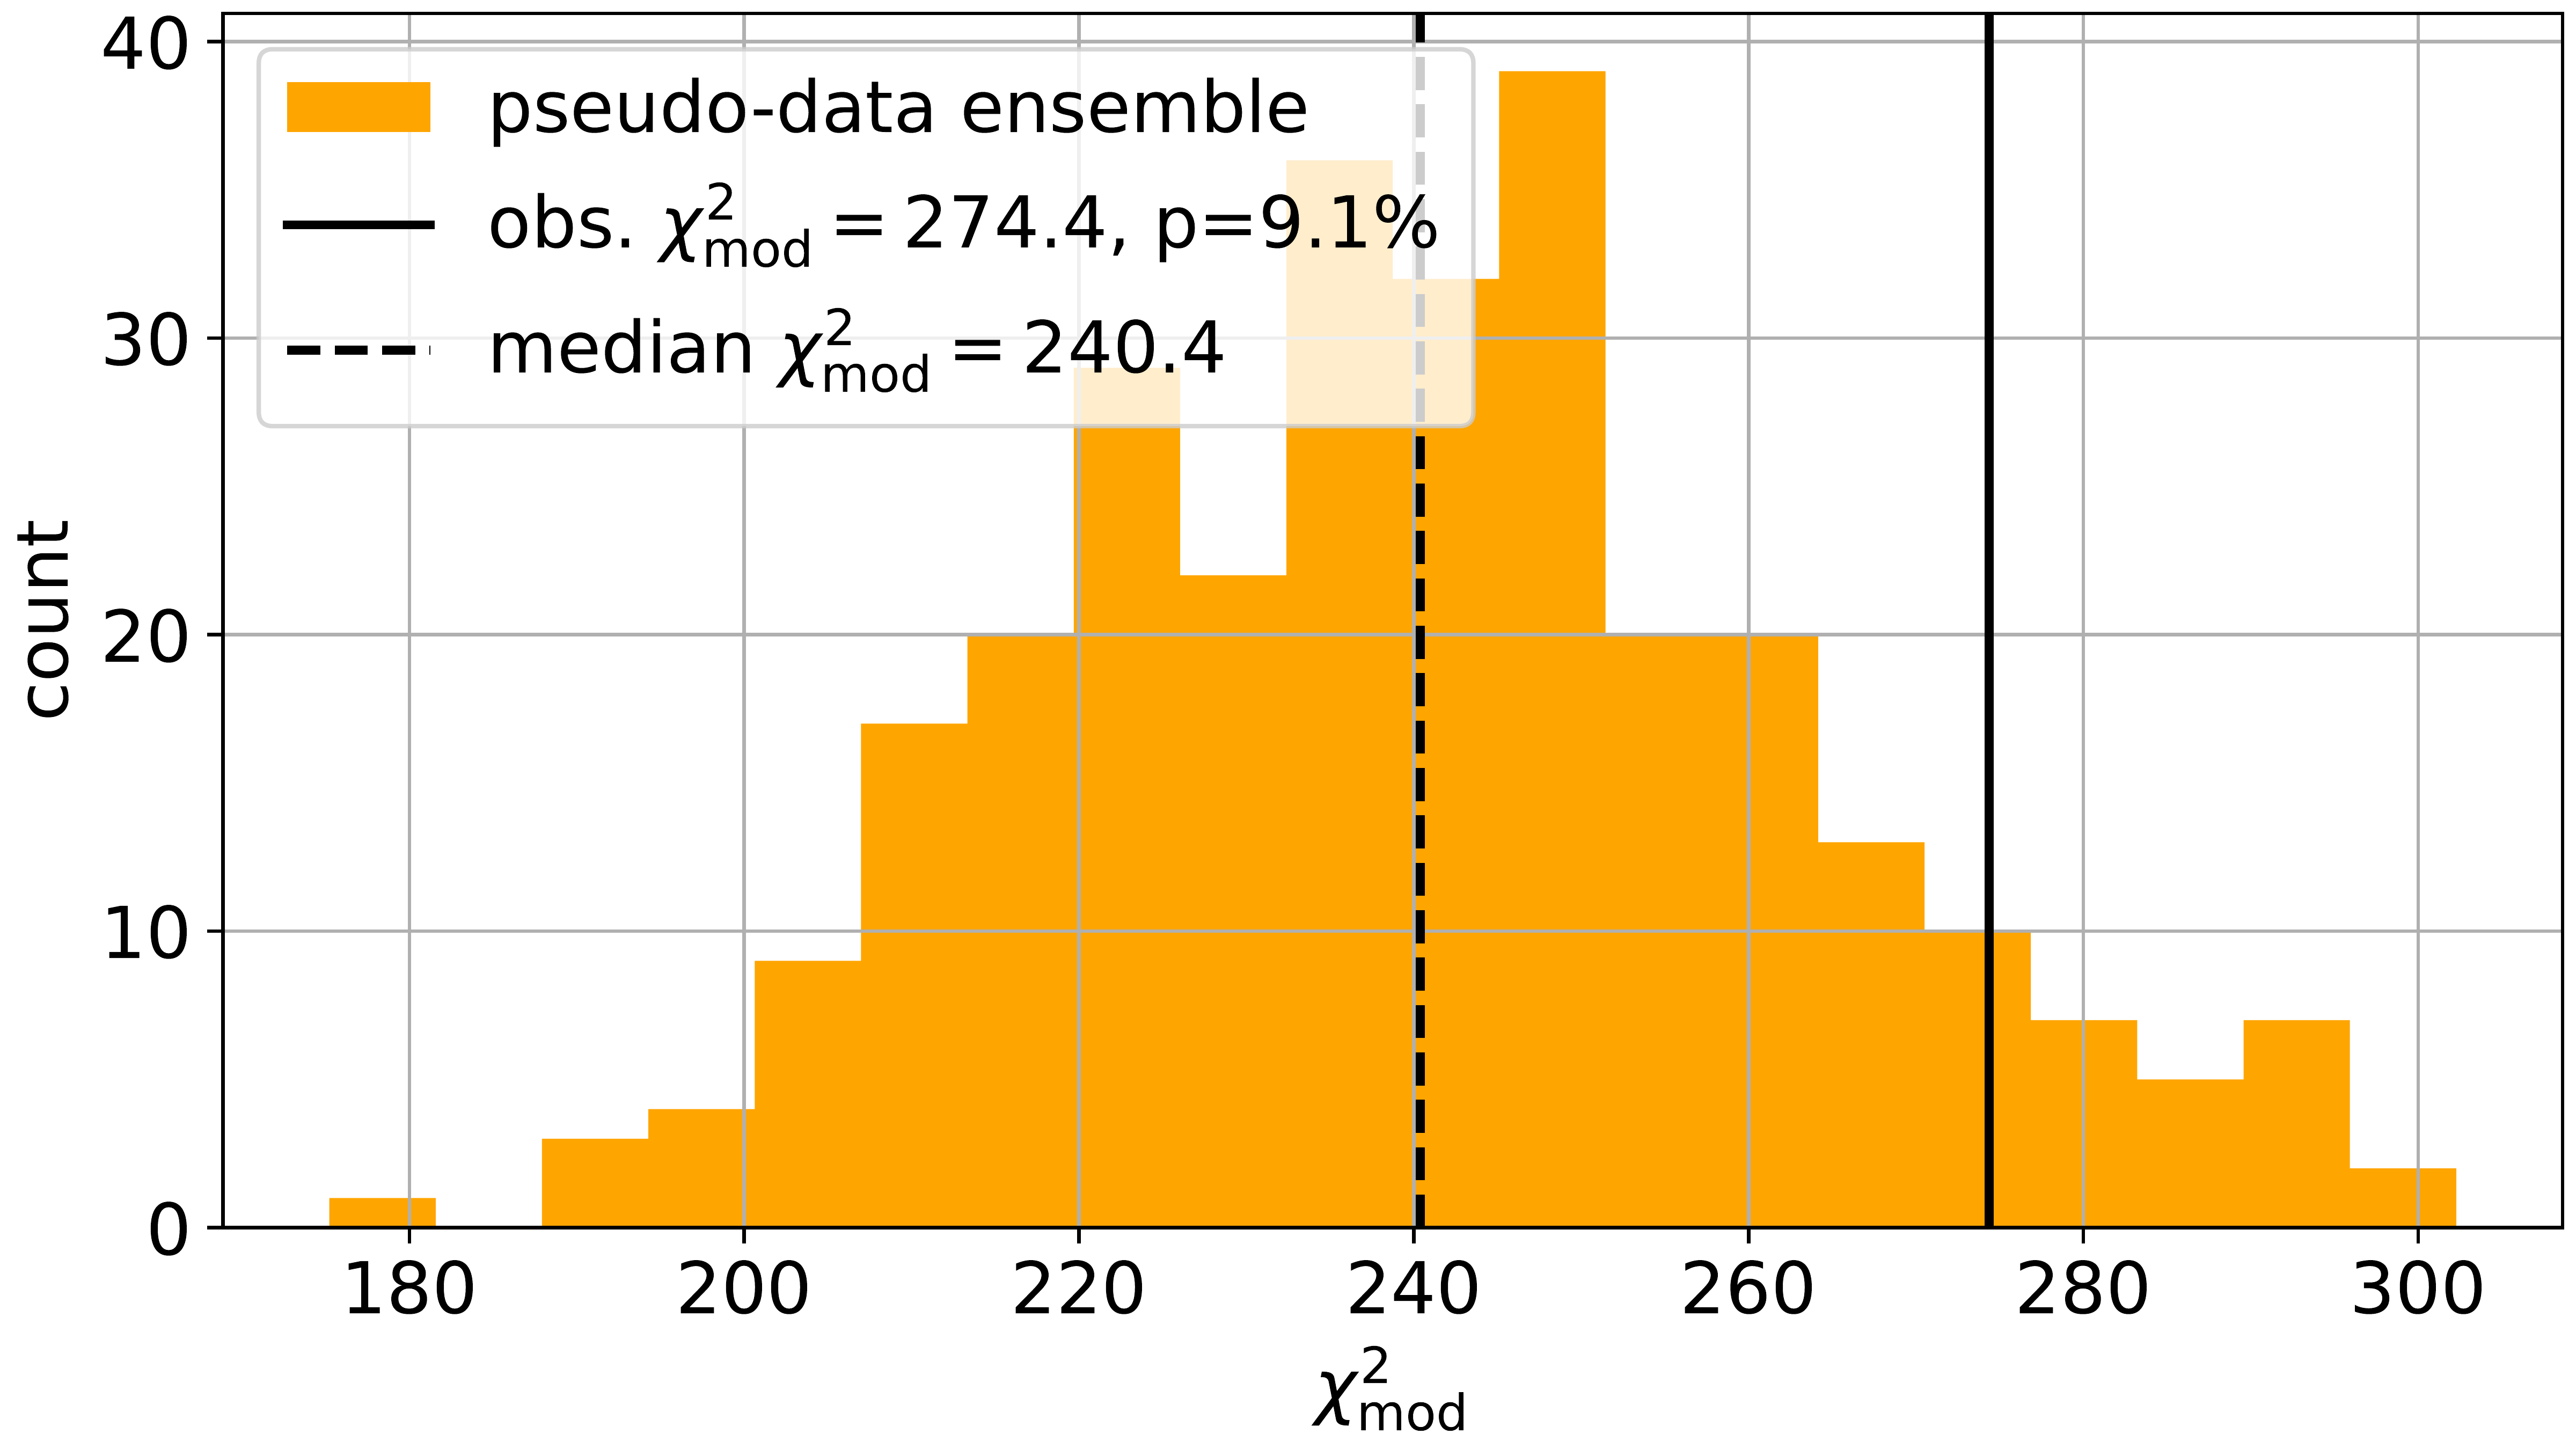
\includegraphics[width=0.49\linewidth]{figures/results/checks/full_blind_fit_1.0_GeV_step_3_4-1.png}
	\caption[Pseudo-data trials TS distribution (\SI{0.3}{\gev}, \SI{1.0}{\gev})]{Observed fit TS and TS distribution from pseudo-data trials for the \SI{0.3}{\gev} (left) and \SI{1.0}{\gev} (right) mass set.}
    \labfig{pseudo_data_ensemble_appendix}
\end{figure*}
